\documentclass[enabledeprecatedfontcommands,fontsize=12pt,paper=a4,twoside]{scrartcl}


\newcommand{\grad}{\ensuremath{^{\circ}} }
\renewcommand{\strut}{\vrule width 0pt height5mm depth2mm}
\usepackage{longtable}
\usepackage[utf8]{inputenc}
\usepackage[T1]{fontenc}
\usepackage[final]{pdfpages}
% obere Seitenränder gestalten können
\usepackage{fancyhdr}
\usepackage{moreverb}
% Graphiken als jpg, png etc. einbinden können
\usepackage{graphicx}
\usepackage[normalem]{ulem}
\useunder{\uline}{\ul}{}
\usepackage{stmaryrd}
% Floats Objekte mit [H] festsetzen
\usepackage{float}
% setzt URL's schön mit \url{http://bla.laber.com/~mypage}
\usepackage{url}
% Externe PDF's einbinden können
\usepackage{pdflscape}
% Verweise innerhalb des Dokuments schick mit " ... auf Seite ... "
% automatisch versehen. Dazu \vref{labelname} benutzen
\usepackage[ngerman]{varioref}
\usepackage[ngerman]{babel}
\usepackage{ngerman}
% Bibliographie
\usepackage{bibgerm}
% Tabellen
\usepackage{tabularx}
\usepackage{supertabular}
\usepackage[colorlinks=true, pdfstartview=FitV, linkcolor=blue,
            citecolor=blue, urlcolor=blue, hyperfigures=true,
            pdftex=true]{hyperref}
\usepackage{bookmark}
\usepackage{rotating}

\hyphenation{Arbeits-paket}

% Damit Latex nicht zu lange Zeilen produziert:
\sloppy
%Uneinheitlicher unterer Seitenrand:
%\raggedbottom

% Kein Erstzeileneinzug beim Absatzanfang
% Sieht aber nur gut aus, wenn man zwischen Absätzen viel Platz einbaut
\setlength{\parindent}{0ex}

% Abstand zwischen zwei Absätzen
\setlength{\parskip}{1ex}

% Seitenränder für Korrekturen verändern
\addtolength{\evensidemargin}{-1cm}
\addtolength{\oddsidemargin}{1cm}

\bibliographystyle{gerapali}

% Lustige Header auf den Seiten
  \pagestyle{fancy}
  \setlength{\headheight}{70.55003pt}
  \fancyhead{}
  \fancyhead[LO,RE]{Software--Projekt 2\\ WiSe 2019/2020
  \\Architekturbeschreibung}
  \fancyhead[LE,RO]{Seite \thepage\\\slshape \leftmark\\\slshape \rightmark}

%Unicode Minuszeichen deklarieren, um es nicht überall austauschen zu müssen
\DeclareUnicodeCharacter{2212}{-}

%
% Und jetzt geht das Dokument los....
%

\begin{document}

% Lustige Header nur auf dieser Seite
  \thispagestyle{fancy}
  \fancyhead[LO,RE]{ }
  \fancyhead[LE,RO]{Universität Bremen\\FB 3 -- Informatik\\
  Prof. Dr. Rainer Koschke \\TutorIn: Marcel Steinbeck}
  \fancyfoot[C]{}

% Start Titelseite
  \vspace{3cm}

  \begin{minipage}[H]{\textwidth}
  \begin{center}
  \bf
  \Large
  Software--Projekt 2 WiSe 2019/2020\\
  \smallskip
  \small
  VAK 03-BA-901.02\\
  \vspace{3cm}
  \end{center}
  \end{minipage}
  \begin{minipage}[H]{\textwidth}
  \begin{center}
  \vspace{1cm}
  \bf
  \Large Architekturbeschreibung\\
  \vfill
  \end{center}
  \end{minipage}
  \vfill
  \begin{minipage}[H]{\textwidth}
  \begin{center}
  \sf
  \begin{tabular}{lr}
  Liam Hurwitz & hurwitz@tzi.de \\
  Kevin Santiago Rodriguez Rey & hurwitz@tzi.de \\
  Fabian Kehlenberg & rudkows@tzi.de \\
  Aaron Rudkowski & rudkows@tzi.de \\
  Samuel nejati Masouleh & rudkows@tzi.de \\
  Leonard Haddad & s\textunderscore xsipo6@tzi.de \\  
\end{tabular}
  \\ ~
  \vspace{2cm}
  \\
  \it Abgabe: 22. Dezember 2019 --- Version 1.0\\ ~
  \end{center}
  \end{minipage}

% Ende Titelseite

% Start Leerseite

\newpage

  \thispagestyle{fancy}
  \fancyhead{}
  \fancyhead[LO,RE]{Software--Projekt \\  2019/2020
  \\Architekturbeschreibung}
  \fancyhead[LE,RO]{Seite \thepage\\\slshape \leftmark\\~}
  \fancyfoot{}
  \renewcommand{\headrulewidth}{0.4pt}
  \tableofcontents

\newpage

  \fancyhead[LE,RO]{Seite \thepage\\\slshape \leftmark\\\slshape \rightmark}


%%%%%%%%%%%%%%%%%%%%%%%%%%%%%%%%%%%%%%%%%%%%%%%%%%%%%%%%%%%%%%%%%%%%%%%%
\section*{Version und Änderungsgeschichte}

{\em Die aktuelle Versionsnummer des Dokumentes sollte eindeutig und gut zu
identifizieren sein, hier und optimalerweise auf dem Titelblatt.}

\begin{tabular}{ccl}
Version & Datum & Änderungen \\
\hline
0.1 & TT.MM.JJJJ & Dokumentvorlage als initiale Fassung kopiert \\
0.2 & 04.12.2019 & Faktortabelle \\
0.3 & 04.12.2019 & Problem Karten \\
\ldots
\end{tabular}


%%%%%%%%%%%%%%%%%%%%%%%%%%%%%%%%%%%%%%%%%%%%%%%%%%%%%%%%%%%%%%%%%%%%%%%%
\section{Einführung}

Diese Architektur Beschreibung wurde im Rahmen von von Software Projekt 2 im Wintersemester 2019/2020 geschrieben. Das Projekt wurde im Rahmen des SFB 1232 Farbige Zustände erstellt. Die SFB-intitative "Farbige Zustände" erarbeitet sich eine neuartige experimentelle Methode der Werkstoffentwicklung.

Es handelt sich hierbei um eine Webapplikation, welche den Mitarbeitern der SFB-Initiative ermöglichen soll, effizient und ohne Verzögerung durch einen Administrativen Mehraufwand Prozessketten für die untersuchten metallischen Konstruktionswerkstoffe zu finden. 
Außerdem ermöglichen wir es den Forschern der SFB-Initative den Überblick über laufende Prozessketten und deren Prozessschritte zu behalten. 
Konkret bedeutet dies, dass wir es den Logistik-beauftragen mit Hilfe unserer Software ermöglichen, Proben und deren Träger zu verwalten. Den Technologen der SFB-Initiative ermöglichen wir es den Überblick über ihre Experimentierstationen zu behalten; sie werden immer über die laufenden Prozessschritte informiert sein.
Dem Prozesskettenadministrator möchten wir es ermöglichen, Prozessketten zu erstellen und verwalten, welche auf digitalem Wege an die Technologen weitergegeben werden als auszuführende Aufträge, welche diese wiederum annehmen und durchführen können.
Außerdem möchten wir den Mitarbeitern im Lager ermöglichen, eine klare Übersicht über die im Lager sich befindende Proben zu behalten.
Außerdem möchten wir dem Transporter der Proben, welcher diese von A nach B transportieren muss, ermöglichen, diese Transporte einfach protokolliert durchführen zu können, mit einfachem Probeverlusts-Protokoll. 
Zu guter Letzt soll es noch dem System-Administrator möglich sein, die Benutzer des Systems zu verwalten und ihnen ihre Rollen im SFB einzuteilen.
 
Diese Webapplikation soll also, in Stichpunkten, die folgenden Funktionen ermöglichen:
\begin{itemize}
  \item Die Erstellung und Verwaltung von Prozessketten durch einen Prozessketten-Administrator.
  \item Eine protokollierte, (digital semi-automatische-) beobachtete Durchführung von Experimenten auf die Werkstoff-Proben. 
  \item Ein protokollierter Transport der Proben in ihren Trägern von A nach B, mit Verlusts-Protokoll.
  \item Eine einfache Übersicht über die im Lager befindende Proben zu haben.
  \item Nutzer der Webapplikation einfach verwalten und ihren Rollen im SFB einteilen zu können.
  \item Das System sollte zudem auch noch lauffähig auf mobilen Geräten sein, und möchte noch auf Englisch verfügbar sein.
\end{itemize}

Leser dieser Architekturbeschreibung sind hiermit also nicht nur die Mitarbeiter der SFB-Initiative, sondern gegeben falls auch der Endkunde, welcher die Benutzer des Systems verwalten kann.

\subsection{Zweck}

  {\em Diese Architekturbeschreibung beschreibt die Architektur von Farbiges SFB, eine digitale Software welche die Erstellung, Verwaltung und Durchführung von Prozessketten ermöglicht, mit wessen Hilfe neue Werkstoffeigenschaften gefunden werden sollen für den industriellen Gebrauch. Es beschreibt wie das System von Farbiges SFB  implementiert werden soll, und wie seine Struktur aussehen wird. 
Dieses Dokument soll allen die die Software bedienen und bearbeiten werden dabei helfen die Struktur und Funktionsweise von Farbiges SFB zu verstehen. Es soll sowohl den Entwicklern eine Übersicht über die Funktionsweise der Software geben, welche diese schließlich implementieren werden, als auch den Testern zur Vorbereitung  ihrer Tests. Es soll außerdem dem Systemadministratoren eine Übersicht der Software geben, da diese das System anschließend verwalten müssen, und diese vielleicht die Software weiterentwickeln möchten. 
}

\subsection{Status}

{\em Diese Architektur beschreibt den ersten Entwurf dieser Software. Es wurde auch noch nicht freigegeben durch ein Architektur Review, und ist somit die allererste Version.  }



\subsection{Definitionen, Akronyme und Abkürzungen}
In diesem Kapitel werden Akronyme und andere Ausdrücke definiert, welche im Laufe des Dokuments verwendet werden.

\begin{longtable}[c]{|p{7cm}|p{8cm}|}
\hline
\multicolumn{1}{|c|}{\textbf{Begriff}}                          & \multicolumn{1}{c|}{\textbf{Erklärung}}                                                                                                                                                                                                               \\ \hline
\endhead
%
\multicolumn{2}{|l|}{{\ul \textbf{Das System Selbst}}}                                                                                                                                                                                                                                                                  \\ \hline
Probe                                                           & Ein einzelnder Werkstoff                                                                                                                                                                                                                              \\ \hline
Werkstoff                                                       & Mikrolkugeln die sich durch Härte, hohe-/Belastbarkeit, Temperaturbeständigkeit und Abriebsfestigkeit auszeichnen                                                                                                                                     \\ \hline
Träger                                                          & Transportmittel für Proben. Arten: Einzelträger, eingebettete Träger und Glasträger. Proben werden immer in Trägern Transportiert                                                                                                                     \\ \hline
Experimentierstation \textbf{(ES)}             & Physikalischer Standort an dem Technologen Messungen durchführen.                                                                                                                                                                                     \\ \hline
Technologe                                                      & Ein Angestellter im SFB, er forscht und bedient die Experimentierstationen, und wertet diese im Anschluss aus und legt die Probeneigenschaften fest.                                                                                                  \\ \hline
Prozesskette \textbf{(PK)}                       & Besteht aus vielen Prozessschritten die hintereinander ohne verzweigung ablaufen. Sobald ein Autrag erfolgt, wird eine Prozesskette gestartet.                                                                                                        \\ \hline
Prozesskettenauftrag \textbf{(PK-Auftrag)}     & Enthält die Prozessparameter für jeden Schritt einer Prozesskette. Der Prozesskettenadministrator legt die Prozessparameter fest. Der Logistiker legt die Proben und Träger fest.                                                                     \\ \hline
Prozessschritt \textbf{(PS)}                     & In einem Prozessschritt werden Werkstoffeigenschaften beeinflußt und-/oder verändert. Er enthält Prozessparameter welche beschreiben wie die Eigenschaften beeinflußt werden. Ein Prozessschritt kann Vorbedingungen haben und eine geschätzte Dauer. \\ \hline
Material- / Werkstoffeigenschaften                              & Jeder Werkstoff besitzt Eingenschaften. (Umformbarkeit / Verformbarkeit / ...)                                                                                                                                                                        \\ \hline
Prozessparameter \textbf{(PP)}                   & Sind Qualitativ oder Quantitativ. Qualitativ beschreibt ob etwas so sit oder nicht. Quantitative Parameter enthalten einen Namen, ein Wert und eine Einheit.                                                                                          \\ \hline
Logistiker                                                      & Verwaltet das Archiv und alle Proben und Träger. Für die Ausführung einer Prozesskette bestimmt er welche Proben benutzt werden, falls dies nicht möglich ist, meldet er es dem Prozesskettenadministrator.                                           \\ \hline
Prozesskettenadministrator\textbf{ (PK-Admin)} & Verwaltet Prozessketten und deren Prozessschritte nach bestimmten Vorlagen. Verwaltet auch die Vorlagen. Ordnet Prozessschritten Experimentierstationen zu. Überprüft dann auf Korrektheit.                                                           \\ \hline
Transporter                                                     & Transportiert Träger mit ihren Proben zwischen Experimentierstationen. Bei Probenverlust meldet er diese.                                                                                                                                             \\ \hline
Transportauftrag \textbf{(T-Auftrag)}          & Enthält Start- und Ziel Experimentierstationen, wird vom Transporter ausgeführt.                                                                                                                                                                      \\ \hline
System Administrator \textbf{(Sys-Admin)}      & Verwaltet Nutzer und Experimentierstationen. Konfiguriert globale Einstellungen und ist für Backup zuständig.                                                                                                                                         \\ \hline
Prozessketteninstanz Werte \textbf{(PIW)}      & Enthält für jeden Prozessschritt der Proezsskette alle Prozessparameter. Der Prozesskettenadmin benutzt die PIWs um Prozessketteninstanzen zu planen.                                                                                                 \\ \hline
Standort                                                        & Träger und Proben können entweder an einer Experimentierstation, im Archiv oder als verloren gemeldet sein.                                                                                                                                           \\ \hline
Transportauftragzustand \textbf{(TA-Zustand)}  & Ein Transportauftrag befindet sich im Zustand wartend oder er wurde schon geliefert.                                                                                                                                                                  \\ \hline
Prozessschrittzustand \textbf{(PS-Zustand)}    & Ein Prozessschrittzustand hat entweder den Zustand angenommen, in-bearbeitung oder abgegeben.                                                                                                                                                         \\ \hline
Upload in Datenbank                                             & Ein Technologe muss nach dem Ausführen eines Prozessschrittes die Prozessparameter in die Datenbank (DAVIS) hochladen.                                                                                                                                \\ \hline
\end{longtable}

\begin{longtable}[c]{|p{7cm}|p{8cm}|}
\hline
\multicolumn{1}{|c|}{\textbf{Begriff}} & \multicolumn{1}{c|}{\textbf{Erklärung}}                                                                                                                                                                                 \\ \hline
\endhead
%
\multicolumn{2}{|l|}{{\ul \textbf{Technische Ausdrücke}}}                                                                                                                                                                                                        \\ \hline
Anwendungsfälle                        & Hilfsmittel um Anforderungen unseres Software-Projektes zu erfassen. Sie beschreiben also, was unser System tun soll. Hierzu nutzen wir Akteuere und Use-Cases.                                                         \\ \hline
H2                                     & Eine SQL Java Datenbank die auch die JDBC API unterstützt.                                                                                                                                                              \\ \hline
Apache Maven                           & Ist ein automatisches Build-tool für Java Projekte. Es beschreibt wie Software gebaut wird und was ihre Dependencies sind.                                                                                              \\ \hline
DAO                                    & Objekte die abstrakte Interfaces zu Datenbanken oder anderen Persistenzmechanismen bieten. Kurzgesagt, werden sie verwendet um Daten aus einer Datenbank zu verwalten (Data Access Object).                             \\ \hline
Java                                   & Eine objektorientierte Programmiersprache, welche klassenbasiert, objekte-orientiert ist. Läuft universell auf fast allen Platformen die eine JVM haben, von PCs zu Handys usw...                                       \\ \hline
JavaEE (JakartaEE)                     & Ist eine Menge an Spezifikationen für Java SE welche Enterprise Features und Webservices sowie Distributed Computation spezifiziert.                                                                                    \\ \hline
Hibernate Validator                    & Ist eine Java Bean Validation referenz Implementation.                                                                                                                                                                  \\ \hline
Lombok                                 & Ist eine Java Bibliothek welche zur automatisierten Code-Erstellung verwendet weden kann (um nicht so viel Code schreiben zu müssen) z.B. automatische Erstellung von Gettern und Settern, Equals, Hashcode und String. \\ \hline
JUnit                                  & Ist eine Unit Testing Framework für Java, zur Überprüfung von bekannten Fehlern in den implementierten Funktionen und Klassen.                                                                                          \\ \hline
Wildfly                                & Ist ein Application Server, der die JavaEE Spezifikation implementiert.                                                                                                                                                 \\ \hline
Mockito                                & Ist ein Mocking Framework für JUnit, zum weiteren Testen der Implementierten Funktionen. Es ermöglicht die Erstellung von Test Double Objekte für automatische Unit Tests.                                              \\ \hline
Scrypt                                 & Eine Passwort basierte Schlüsselableitungsfunktion die nicht umkehrbar ist.                                                                                                                                             \\ \hline
Bootsfaces                             & Ist eine JSF Framework welche Bootstrap und JQuery benutzt um responsive Front-Ends zu entwickeln.                                                                                                                      \\ \hline
Primefaces                             & Ist eine Menge an UI Komponenten für JSF. Es bietet Templates und Themes an.                                                                                                                                            \\ \hline
JSF                                    & Steht für Java Server Faces. Ist eine Spezifikation zur Entwicklung von graphischen Oberflächen in Java.                                                                                                                \\ \hline
GUI                                    & Eine Form eines Benutzer Interfaces, die dem Benutzer erlaubt durch elektronische Geräte graphisch mit der Software zu enteragieren (Graphical User Interface).                                                         \\ \hline
Klassendiagramm                        & Ist ein Typ von statischen Struktur Diagrammen, welche Klassen, Attribute, Operationen und Relationen des Systems als Diagramm darstellen.                                                                              \\ \hline
Komponentendiagramm                    & Beschreiben wie Komponenten durch ihre Schnittstellen verbunden sind. Sie werden benutzt um die Struktur komplexer Systeme darzustellen.                                                                                \\ \hline
Model-View-Controller (MVC)            & Ein Architekturmuster welches für User Interfaces benutzt wird um Programmlogik in 3 Elemente zu unterteilen: Model, View und Controller.                                                                               \\ \hline
Object-Relation-Mapping (ORM)          & ===TODO====                                                                                                                                                                                                             \\ \hline
Packetdiagramm                         & Zeigt die Abhängigkeiten der Packete des Models.                                                                                                                                                                        \\ \hline
Sequenzdiagramme                       & Zeigt die Struktur unseres Models und stellt den Austausch von nachricten zwischen Objekten dar. Dabei wird eine Lebenslinie benutzt.                                                                                   \\ \hline
Problemkarten                          & Beschreiben Probleme und passende Strategien.                                                                                                                                                                           \\ \hline
SQL                                    & Ist eine domän spezifische Sprache die in der Softwareentwicklung benutzt wird und Daten in relationalen Datenbanken verwaltet.                                                                                         \\ \hline
\end{longtable}
\subsection{Referenzen}
\begin{itemize}
  \item Architekturbeschreibung von RainersRaiders im Rahmen von Softwareprojekt 2 - 2016
  \item Kickoff Folien
\end{itemize}
\subsection{Übersicht über das Dokument}

{ \em Im Kapitel 2 werden wir zunächst verschiedene Anwendungsfälle unserer Software beschreiben, welche wir als Ausgangspunkt für unsere Architekturstruktur verwenden werden. In Kapitel 3 werden die Einflussfaktoren und Probleme und Strategien, die zum Lösen der Probleme entworfen wurden, dargestellt.
In den Kapiteln 4, 5 und 7 werden die verschiedenen Sichten von Hofmeister gezeigt. Die Codesicht wird in diesem Projekt nicht behandelt.
Im Nachfolgenden Kapitel 4 wird die Konzeptionelle Sicht unserer Software beschrieben. In Kapitel 5 wird die Modulsicht und In Kapitel 7 wird die Ausführungssicht gezeigt. Kapitel 6 ist eine nähere Beschreibung der Architektursicht und wird durch ein Modell in der Datensicht dargestellt.
Im Kapitel 8 werden einige Anwendungsfälle dargestellt. im abschließenden Kapitel 9 wird auf die mögliche zukünftige Entwicklung der Software bei neu eingehenden Wünschen der Kunden eingegangen.

}


%%%%%%%%%%%%%%%%%%%%%%%%%%%%%%%%%%%%%%%%%%%%%%%%%%%%%%%%%%%%%%%%%%%%%%%

\section{Anwendungsfälle}

In diesen Kapitel werden wir verschiedene Anwendungsszenarien abdecken, welche unsere Software erfüllen soll. Diese Szenarien werden wir als Ausgangs- und Vergleichspunkt für den Rest unserer Architektur benutzen. Hiermit kann am Ende geprüft werden, ob die Software alle Anforderungen erfüllt. 

\subsection{Anmeldung am System (alle Benutzer)}

Der Benutzer wird mit einem Login-Fenster begrüßt an welchem er sich einloggen kann. Sollte es noch keinen Benutzer im System geben, so kann ein neuer Benutzer über ein Create-Account Knopf erstellt werden. Sollte er sein Passwort vergessen haben, so kann er mithilfe von einem Passwort Vergessen Knopf dieses zurücksetzen.
Nach der Erstellung eines Benutzers wird dieser im Datenbanksystem eingespeichert, wodurch der System Administrator ihm nun eine Rolle einteilen kann.
Der System Administrator befindet sich schon zu Anfang im System. Das heißt er muss seinen Benutzer nicht neu erstellen.
Nach einer erfolgreichen Anmeldung am System werden alle Benutzer mit einer Navigationstabelle begrüßt. Diese Tabelle beinhaltet die für den Benutzer spezifizierten Funktionalitäten.

\subsection{Benutzer Verwaltung - System Administrator}

Die Aufgabe des System Administrators ist es die Benutzer zu verwalten. Nach seiner Anmeldung am System wird dieser mit einer Tabelle begrüßt welche seine Optionen im System anzeigt. Nach druck auf den Knopf für Nutzerverwaltung wird er mit einer weiteren Tabelle begrüßt, welche alle Nutzer des Systems beinhaltet. Diese Tabelle hat sowohl einen sortierungs Knopf, als auch eine Suchbox, wodurch er die angezeigten Nutzer des Systems filtern kann.
Jeder Nutzer hat einen Bearbeitungsknopf neben seinem Namen. Durch druck auf diesen Knopf öffnet sich ein weiteres Fenster, in dem der Systemadministrator alle Optionen zur Verwaltung des Nutzers hat. Hier kann er z.B. dessen Details ändern (Name, Vorname, usw...), seine Rolle im SFB (Technologe, Transporter, usw...), aber auch einen Löschung Knopf mit welchem er diesen Benutzer aus dem System entfernen kann. 
Die Tabelle beinhaltet natürlich auch einen Add Knopf, wodurch der System Administrator neue Benutzer im System einfügen kann. 

\subsection{Experimentierstationsverwaltung - System Administrator}

Wir nehmen an der Administrator hätte sich schon im System angemeldet. In dem vor ihm stehendes Fenster sieht er unter der Benutzerverwaltung einen weiteren Knopf zur Experimentierstationsverwaltung. Durch druck auf diesen Knopf öffnet sich ein weiteres Fenster mit einer weiteren Tabelle welche alle im System enthaltenden Experimentierstationen beinhaltet.  Diese sind auch wieder mal in reihen der Tabelle eingeteilt. Jede Reihe hat rechts einen Knopf mit welchem der Administrator die zugehörige Experimentierstation verwalten kann, und daneben einen weiteren Knopf zur Löschung der Experimentierstation.
Unten in der Tabelle befindet sich ein weiterer Knopf mit welchem er weitere Experimentierstationen einfügen kann.
Bei normalen druck auf eine Experimentierstation werden Informationen über diese angezeigt, wie z.B. Standort und ob diese momentan in Benutzung ist. 
  
\subsection{Prozesskettenverwaltung - Prozesskettenadministrator}

Da die Aufgabe des Prozesskettenadministrators die Erstellung und Verwaltung von Prozessketten ist, wird dieser nach seiner Anmeldung am System mit einem Fenster begrüßt, wo er durch druck auf den Knopf zur Prozesskettenverwaltung mit einem weiteren Fenster begrüßt wird, welches alle Prozessketten des Systems enthält.
Auch diese Tabelle kann durch eine Suchbox und weitere Kriterien wie z.B. Datum der Erstellung der Prozesskette filtriert werden.
In dieser Tabelle sind alle Prozessketten die sich im System befinden, in reihen sortiert, sichtbar. An der Seite jeder noch nicht instanziierten Prozesskette ist ein Knopf um diese zu Bearbeiten. Durch druck auf den Bearbeitungsknopf kann der Prozesskettenadministrator die Schritte dieser Prozesskette bearbeiten. Hier kann er z.B. weitere Schritte der Prozesskette hinzufügen, oder schon existierende Schritte entfernen.
Ein weiterer Knopf in der Tabelle erlaubt ihm eine Prozesskette zu starten. Sobald dieses getan ist, kann diese nicht mehr von ihm gestoppt werden.
Die Tabelle beinhaltet auch einen Einfügungs-Knopf, durch welchen weitere Prozessketten erstellt werden können.
Bei Erstellung einer Prozesskette wird diese auf Korrektheit überprüft. Sollte ein Prozessschritt z.B. unrealistische Vorbedingungen haben, so wird dem Prozesskettenadministrator Bescheid gegeben, dass er diese Prozesskette im jetzigen Stand nicht erstellen kann.
Bei der Erstellung von Prozessketten, welche aus verschiedenen Prozessschritten besteht, muss der Prozesskettenadministrator natürlich auch diese Prozessschritte erstellen. Bei der Erstellung von Prozessketten wird er also mit einem Fenster begrüßt in welchem er die Prozessschritte der Prozesskette verwalten kann.
Hier kann er z.B. einem Prozessschritt Vorbedingungen geben, welche er in einem Vorbedingungsfeld eingeben kann. In einem weiteren Feld kann er die Experimentierstation dieses Schrittes zuordnen. Diese Prozessschritte kann er so lange noch bearbeiten und verändern, bis die Prozesskette gestartet wird, durch den druck auf den Knopf zur Bearbeitung der Prozesskette. 
Sollte eine Prozesskette in Bearbeitung sein, so kann der Prozesskettenadministrator auf diese drücken um zu sehen bei welchem Schritt sie sich momentan befindet. Er kann außerdem auch alle schon abgelaufenen- und noch auszuführende-Schritte sehen.
 
\subsection{Lagerübersicht - Logistiker}

Nehmen wir an der Logistiker hätte sich im System schon angemeldet.
In dem von ihm befindenden Fenster ist ein Knopf für Lagerübersicht. Durch druck auf diesen öffnet sich ein weiteres Fenster mit einer Tabelle welche alle sich im Lager befindenden Proben beinhaltet. Auch diese Tabelle kann durch Suchbox und weiteres filtriert werden. Sie beinhaltet aber auch eine Option zur Gruppierung der Proben nach Legierung, Wärmebehandlung und Stationen.

\subsection{Proben mit Prozessketten assoziieren - Logistiker}

Nach seinem Login findet der Logistiker in dem Begrüßungsfenster ein weiteren Knopf für Prozessketten. Hier kann er die verschiedenen Prozessketten sehen welche gerade ausgeführt werden und welche Proben sie benötigen. Durch eine schnelle suche mit z.B. der Suchbox im Lagerübersichtsfenster kann der Logistiker herausfinden, ob die benötigten Proben sich im Lager befinden. Es soll bei jeder Prozesskette auch einen automatisierten Suchknopf geben welcher diese Proben automatisch im Lager sucht.
Befinden sich die Proben im Lager, so kann er die Proben der Prozesskette zuweisen. Sollte das nicht der Fall sein, so kann er auf einen Knopf neben der Prozesskette drücken, wodurch dem Prozesskettenadministrator Bescheid gegeben wird das die benötigten Proben nicht verfügbar sind.
 
\subsection{Prozessketten Starten/Stoppen - Logistiker}

Sollten die benötigten Proben vom Letzten Absatz sich im Lager befinden, so kann der Logistiker durch einen weiteren Knopf eine noch nicht gestartete Prozesskette starten.
Sollte aus welchem Grund auch immer eine Prozesskette gestoppt werden, so kann dieser auch diese stoppen.

\subsection{Zustand eines Auftrags angeben - Technologe}

Nehmen wir an der Technologe hätte sich schon im System angemeldet. Er sieht vor sich ein Fenster mit einem Knopf für Aufträge. Durch druck auf diesen gelangt er zu einem weiteren Fenster in dem alle verfügbaren Aufträge als Reihen in einer Tabelle angezeigt werden. Hier kann er nun einen Auftrag annehmen, durch druck auf einen Knopf neben einem Auftrag, wodurch dieser Auftrag automatisch in den Zustand angenommen geht. Dieser Auftrag kann nun von keinem anderen Technologen mehr angenommen werden. Sobald der Technologe mit der Bearbeitung des Auftrags beginnt, muss er nur auf den Knopf für in-Bearbeitung drücken, wodurch dieser Auftrag nun automatisch in den Zustand in-Bearbeitung gelangt. Sobald der Technologe mit seiner Bearbeitung fertig ist, muss er nur auf einen Knopf drücken, wodurch der Auftrag nun als Bearbeitet gekennzeichnet wird. Sollte er nun diesen Auftrag weiterschicken möchten, so kann er dieses durch druck auf einen weiteren Knopf tun. Sobald der Technologe die Prozessparameter dieses Auftrags in der Datenbank hochgeladen hat, wird der Auftrag entweder automatisch auf in die DB hochgeladen gesetzt, oder manuell durch den Technologen. Dieses kommt drauf an ob der Technologe zum Hochladen der Daten den Knopf in diesem Auftrag verwendet hat, oder einen anderen.

\subsection{Aufnahme der Zeit in einem Auftrag - Technologe}

Bei der Annahme eines Auftrags aus dem  vorherigen Absatz wird die jetzige Systemzeit aufgenommen und im Auftrag eingegeben. Das gleiche passiert auch bei den weiteren Schritten aus dem vorherigen Absatz.
Sollte der Technologe allerdings an einem späteren Zeitpunkt diese Zeiten bearbeiten möchten, so kann er durch druck auf einen Bearbeitungsknopf neben dem Auftrag in der Tabelle die Zeiten manuell ändern.  

\subsection{Station Fehler Melden - Technologe}

Sollte irgendetwas schiefgehen und eine Station fehlerhaft werden, so kann der Technologe, nach seiner Anmeldung im System, durch einen Knopf einen Station Fehler melden. Hierdurch wird das System auch die Fehlernachricht bekommen, und somit allen anderen Prozessketten welche diese Station benötigen darüber Bescheid geben. 

\subsection{Proben Transportieren - Transporter}

Nehmen wir an der Transporter hätte sich schon am System angemeldet. Er sieht ein Fenster mit einem Transportübersicht Knopf, welcher ein weiteres Fenster öffnet, mit allen Transportaufträgen als Reihen in einer Tabelle. Hier kann er, durch druck auf einen Auftrag sehen, wo diese Proben abgeholt werden müssen, und wo sie hin geliefert werden müssen. 
Er kann durch Knopfdruck einen Auftrag annehmen, wodurch dieser als Annahme gekennzeichnet wird. Sobald er die Proben abgeholt hat, kann er durch Knopfdruck diesen Auftrag auf die Kennzeichnung Transport setzen. Sobald er die Proben zum korrekten Ort gebracht hat, kann er durch einen weiteren Knopfdruck diesen Auftrag als Ausgeliefert markieren.

\subsection{Probenverlust Melden - Transporter}

Nachdem der Transporter den Transport aus dem vorherigen Abschnitt ausgeführt hat, kann er durch druck auf einen Knopf innerhalb der Auftragstabelle für jeden Auftrag Probenverlust angeben. Hierdurch wird der Auftrag automatisch auf den Zustand Verlust gesetzt.


\section{Globale Analyse}

\label{sec:globale_analyse}

{\it Hier werden Einflussfaktoren aufgezählt und bewertet sowie Strategien
zum Umgang mit interferierenden Einflussfaktoren entwickelt.}

%%%%%%%%%%%%%%%%%%%%%%%%%%%%%%%%%%%%%%%%%%%%
\subsection{Einflussfaktoren}


%\label{sec:einflussfaktoren}
%{\it Hier sind Einflussfaktoren gefragt, die sich auf die Architektur
 % beziehen. Es sind ausschließlich architekturrelevante
 % Einflussfaktoren, und nicht z.\,B.\ solche, die lediglich einen
 % Einfluss auf das Projektmanagement haben. Fragt Euch also bei jedem
 % Faktor: Beeinflusst er wirklich die Architektur? Macht einen
 % einfachen Test: Wie würde die Architektur aussehen, wenn ihr den
 % Einflussfaktor E berücksichtigt? Wie würde sie aussehen, wenn Ihr E nicht
 % berücksichtigt? Kommt in beiden Fällen dieselbe Architektur heraus,
 % dann kann der Einflussfaktor nicht architekturrelevant sein.

  %Es geht hier um Einflussfaktoren, die
  %\begin{enumerate}
  %\item sich über die Zeit ändern,
  %\item viele Komponenten betreffen,
  %\item schwer zu erfüllen sind oder
  %\item mit denen man wenig Erfahrung hat.
  %\end{enumerate}
  %Die Flexibilität und Veränderlichkeit müssen ebenfalls charakterisiert werden.
  %\begin{enumerate}
  %\item Flexibilität: Könnt Ihr den Faktor zum jetzigen Zeitpunkt beeinflussen?
  %\item Veränderlichkeit: ändert der Faktor sich später durch äußere Einflüsse?
%\end{enumerate}

  %Unter Auswirkungen sollte dann beschrieben werden, {\em wie} der
  %Faktor {\em was} beeinflusst. Das können sein:
  %\begin{itemize}
  %\item andere Faktoren
  %\item Komponenten
  %\item Operationsmodi
  %\item Designentscheidungen (Strategien)
  %\end{itemize}

  %Verwendet eine eindeutige Nummerierung der Faktoren, um sie auf den
  %Problemkarten einfach referenzieren zu können.  }
  %%%%%%%%%%%%%%%%%%
\begin{table}[H]
\centering
\begin{tabular}{|p{1cm}|p{3cm}|p{5cm}|p{1cm}|p{5cm}|}
\hline
\begin{tabular}[c]{@{}l@{}}Abge-\\ leitet\\aus\end{tabular} & Einflussfaktor                                                                        & \begin{tabular}[c]{@{}l@{}}Flexibilität und \\ Veränderlichkeit\end{tabular}                                                              & \begin{tabular}[c]{@{}l@{}}++/\\\\ −−\end{tabular} & Auswirkungen                                                                                                                                                                                                                              \\ \hline
\multicolumn{5}{|l|}{O1 : Organisation}                                                                                                                                                                                                                                                                                                                                                                                                                                                                                                                                                          \\ \hline
\multicolumn{5}{|l|}{O1.1 Time-To-Market}                                                                                                                                                                                                                                                                                                                                                                                                                                                                                                                                                        \\ \hline
                                                          & \begin{tabular}[c]{@{}l@{}}Die Auslieferung\\  erfolgt am\\  08.03.2020.\end{tabular} & \begin{tabular}[c]{@{}l@{}}Keine Flexibilität, da\\   Vorgaben bestehen. /\\   Keine Veränderbarkeit, da\\  Vorgaben bestehen.\end{tabular} & \begin{tabular}[c]{@{}l@{}}−−/\\   −−\end{tabular} & \begin{tabular}[c]{@{}l@{}}Nicht alle\\  Funktionen können\\  realisiert werden.\end{tabular}                                                                                                                                             \\ \hline
\multicolumn{5}{|l|}{O1.2 Architektur-Abgabe}                                                                                                                                                                                                                                                                                                                                                                                                                                                                                                                                                    \\ \hline
                                                          & \begin{tabular}[c]{@{}l@{}}Die Auslieferung \\erfolgt am\\ 22.12.2020.\end{tabular}      & \begin{tabular}[c]{@{}l@{}}Keine Flexibilität, da\\   Vorgaben bestehen. /\\   Keine Veränderbarkeit, da\\  Vorgaben bestehen.\end{tabular} & \begin{tabular}[c]{@{}l@{}}−−/\\   −−\end{tabular} & \begin{tabular}[c]{@{}l@{}}Durch den\\ Zeitdruck könnte\\ die Architektur\\ mangelhaft\\ werden. Wenn wir\\ uns nicht genug\\ Zeit lassen,\\ könnten Aspekte,\\ die relevant für die\\ Architektur sind,\\ vergessen werden.\end{tabular} \\ \hline
\multicolumn{5}{|l|}{O1.3 Entwickler}                                                                                                                                                                                                                                                                                                                                                                                                                                                                                                                                                    \\ \hline
                                                          & \begin{tabular}[c]{@{}l@{}}Die\\ Projektgruppe \\besteht aus\\ 6 Entwicklern\\\end{tabular}      & \begin{tabular}[c]{@{}l@{}}Keine Flexibilität, da\\   Vorgaben bestehen. /\\   Keine Veränderbarkeit, da\\  Vorgaben bestehen.\end{tabular} & \begin{tabular}[c]{@{}l@{}}−−/\\   −−\end{tabular} & \begin{tabular}[c]{@{}l@{}}Mangel an der Architektur\\ \end{tabular} \\ \hline

\multicolumn{5}{|l|}{O1.4 Fähigkeiten Entwickler}                                                                                                                                                                                                                                                                                                                                                                                                                                                                                                                                                    \\ \hline
                                                          & \begin{tabular}[c]{@{}l@{}}Nicht alle \\ Entwickler \\ haben die gleiche \\ Programmier-\\erfahrung \\ und auch nicht \\ mit den gleichen \\ Technologien. \end{tabular}      & \begin{tabular}[c]{@{}l@{}}Hohe \\ Veränderlichkeit \\durch Ausführen des\\ Projekts und \\Recherche. \end{tabular} & \begin{tabular}[c]{@{}l@{}}−−/\\   −−\end{tabular} & \begin{tabular}[c]{@{}l@{}}Die Implementierung \\ kann Mangel enthalten. \\\end{tabular} \\ \hline

\end{tabular}
\end{table}

\begin{table}[H]
\centering
\begin{tabular}{|p{1cm}|p{3cm}|p{5cm}|p{1cm}|p{5cm}|}
\hline
\begin{tabular}[c]{@{}l@{}}Abge-\\ leitet\\aus\end{tabular} & Einflussfaktor                                                                        & \begin{tabular}[c]{@{}l@{}}Flexibilität und \\ Veränderlichkeit\end{tabular}                                                              & \begin{tabular}[c]{@{}l@{}}++/\\\\ −−\end{tabular} & Auswirkungen                                                                                                                                                                                                                              \\ \hline
\multicolumn{5}{|l|}{T1: Technik}
\\ \hline
\multicolumn{5}{|l|}{T1.1: Programmiersprache}                                                                                                                                                                                                                                                                                                                                                                                                                                                                                                                                                    \\ \hline
                                                          & \begin{tabular}[c]{@{}l@{}}Java 11 \\ oder höher ist \\ vorgegeben.\end{tabular}      & \begin{tabular}[c]{@{}l@{}}Ein wenig Flexibilität \\ an der Version \\ der Sprache aber \\ nicht an der \\ Sprache.\end{tabular} & \begin{tabular}[c]{@{}l@{}}−−/\\   −−\end{tabular} & \begin{tabular}[c]{@{}l@{}}Das Projekt muss\\ in Java umgesetzt \\werden.\end{tabular} \\ \hline

\multicolumn{5}{|l|}{T1.2 Webbrowser}                                                                                                                                                                                                                                                                                                                                                                                                                                                                                                                                                    \\ \hline
                                                          & \begin{tabular}[c]{@{}l@{}}Die Anwendung \\muss in gängigen \\Browsern \\(Firefox,\\ Internet Explorer, \\Safari, Edge) \\ laufen. \end{tabular}      & \begin{tabular}[c]{@{}l@{}}Keine Flexibilität, da\\   Vorgaben bestehen. /\\   Keine Veränderbarkeit, da\\  Vorgaben bestehen.\end{tabular} & \begin{tabular}[c]{@{}l@{}}−−/\\   −−\end{tabular} & \begin{tabular}[c]{@{}l@{}}Bei der Implementierung \\ muss darauf geachtet \\ werden, \\plattformunabhängig \\ vorzugehen. \end{tabular} \\ \hline

\multicolumn{5}{|l|}{T1.3 Server}                                                                                                                                                                                                                                                                                                                                                                                                                                                                                                                                                    \\ \hline
                                                          & \begin{tabular}[c]{@{}l@{}}Zur\\ Implementierung\\ muss JavaEE 8\\ benutzt werden. \end{tabular}      & \begin{tabular}[c]{@{}l@{}}Keine Flexibilität, da\\   Vorgaben bestehen. /\\   Keine Veränderbarkeit, da\\  Vorgaben bestehen.\end{tabular} & \begin{tabular}[c]{@{}l@{}}−−/\\   −−\end{tabular} & \begin{tabular}[c]{@{}l@{}}Das Projekt\\ muss komplett \\in Java \\umgesetzt werden.\end{tabular} \\ \hline

\multicolumn{5}{|l|}{T1.4: Oberfläche}                                                                                                                                                                                                                                                                                                                                                                                                                                                                                                                                                    \\ \hline
                                                          & \begin{tabular}[c]{@{}l@{}}Als Framework \\zur Erstellung \\der Oberfläche\\ muss JSF\\ verwendet\\ werden.\end{tabular}      & \begin{tabular}[c]{@{}l@{}}Keine Flexibilität, da\\   Vorgaben bestehen. /\\   Keine Veränderbarkeit, da\\  Vorgaben bestehen.\end{tabular} & \begin{tabular}[c]{@{}l@{}}−−/\\   −−\end{tabular} & \begin{tabular}[c]{@{}l@{}}Das Projekt muss\\ in Java umgesetzt \\werden.\end{tabular} \\ \hline

\multicolumn{5}{|l|}{T1.5: Persistenz}                                                                                                                                                                                                                                                                                                                                                                                                                                                                                                                                                    \\ \hline
                                                          & \begin{tabular}[c]{@{}l@{}}Relationale\\ Datenbank H2 \\muss für die\\ Persistenz\\ verwendet werden.\end{tabular}      & \begin{tabular}[c]{@{}l@{}}Keine Flexibilität, da\\   Vorgaben bestehen. /\\   Keine Veränderbarkeit, da\\  Vorgaben bestehen.\end{tabular} & \begin{tabular}[c]{@{}l@{}}−−/\\   −−\end{tabular} & \begin{tabular}[c]{@{}l@{}}Bei der Implementierung\\muss H2 verwendet \\werden.\end{tabular} \\ \hline

\multicolumn{5}{|l|}{T1.6: Build System}                                                                                                                                                                                                                                                                                                                                                                                                                                                                                                                                                    \\ \hline
                                                          & \begin{tabular}[c]{@{}l@{}}Maven\\ muss als\\ Build-System \\verwendet werden.\end{tabular}      & \begin{tabular}[c]{@{}l@{}}Keine Flexibilität, da\\   Vorgaben bestehen. /\\   Keine Veränderbarkeit, da\\  Vorgaben bestehen.\end{tabular} & \begin{tabular}[c]{@{}l@{}}−−/\\   −−\end{tabular} & \begin{tabular}[c]{@{}l@{}}Das Projekt muss\\ maven-build\\ fähig sein.\\\end{tabular} \\ \hline
\end{tabular}
\end{table}

\begin{table}[H]
\centering
\begin{tabular}{|p{1cm}|p{3cm}|p{5cm}|p{1cm}|p{5cm}|}
\hline
\begin{tabular}[c]{@{}l@{}}Abge-\\ leitet\\aus\end{tabular} & Einflussfaktor                                                                        & \begin{tabular}[c]{@{}l@{}}Flexibilität und \\ Veränderlichkeit\end{tabular}                                                              & \begin{tabular}[c]{@{}l@{}}++/\\\\ −−\end{tabular} & Auswirkungen                                                                                                                                                                                                                              \\ \hline
\multicolumn{5}{|l|}{T1.7: Multiple Users}                                                                                                                                                                                                                                                                                                                                                                                                                                                                                                                                                    \\ \hline
                                                          & \begin{tabular}[c]{@{}l@{}}Die Anwendung\\ muss von \\mehreren\\ Benutzern \\gleichzeitig\\ verwendbar sein.\end{tabular}      & \begin{tabular}[c]{@{}l@{}}Keine Flexibilität, da\\   Vorgaben bestehen. /\\   Keine Veränderbarkeit, da\\  Vorgaben bestehen.\end{tabular} & \begin{tabular}[c]{@{}l@{}}−−/\\   −−\end{tabular} & \begin{tabular}[c]{@{}l@{}}Die Anwendung\\ darf nicht von\\ gleichzeitiger \\Verwendung von\\ mehreren Nutzern\\ überfordert sein;\\ ebenfalls dürfen \\dadurch keine\\ Sicherheitslücken \\entstehen.\end{tabular} \\ \hline
\multicolumn{5}{|l|}{P1: Produktfaktoren}
\\ \hline
\multicolumn{5}{|l|}{P1.1: Produktfunktionen}
\\ \hline
\multicolumn{5}{|l|}{P1.1.1: Upload}                                                                                                                                                                                                                                                                                                                                                                                                                                                                                                                                                    \\ \hline
                                                          & \begin{tabular}[c]{@{}l@{}}Prozessketten-\\ und \\Prozessschritte \\Parameter\\ sollen aus \\JSON-Dateien\\ hochgeladen \\werden können. \end{tabular}      & \begin{tabular}[c]{@{}l@{}}Keine\\ Veränderlichkeit,\\ da es vom Chinese \\Menu ist aber\\ Flexibilität gegeben:\\ muss nicht\\ unbedingt gemacht werden.\end{tabular} & \begin{tabular}[c]{@{}l@{}}−−/\\   −−\end{tabular} & \begin{tabular}[c]{@{}l@{}}Die Architektur\\ muss vorsehen,\\ dass JSON-Dateien\\ hochgeladen \\werden können, aus\\ denen automatisch für \\einen Prozessschritt/\\eine Prozesskette \\die Parameter\\ eingefügt werden.\end{tabular} \\ \hline

\multicolumn{5}{|l|}{P1.1.2: Download}                                                                                                                                                                                                                                                                                                                                                                                                                                                                                                                                                    \\ \hline
                                                          & \begin{tabular}[c]{@{}l@{}}Die Parameter \\von einzelnen \\Prozessschritten \\sollen nach JSON \\exportiert und \\heruntergeladen \\werden können. \end{tabular}      & \begin{tabular}[c]{@{}l@{}}Keine\\ Veränderlichkeit,\\ da es vom Chinese \\Menu ist aber\\ Flexibilität gegeben:\\ muss nicht\\ unbedingt gemacht werden.\end{tabular} & \begin{tabular}[c]{@{}l@{}}−−/\\   −−\end{tabular} & \begin{tabular}[c]{@{}l@{}}Die Architektur muss \\vorsehen, dass für einen\\ Prozessschritt \\die Parameter gelistet\\ und in einem JSON-Format\\ exportiert werden können.\end{tabular} \\ \hline

\multicolumn{5}{|l|}{P1.2: Protokollierung}                                                                                                                                                                                                                                                                                                                                                                                                                                                                                                                                                    \\ \hline
                                                          & \begin{tabular}[c]{@{}l@{}}Die Übergänge \\in den \\Prozessketten\\ müssen\\ protokolliert\\ werden.\\ \end{tabular}      & \begin{tabular}[c]{@{}l@{}}Keine\\ Veränderlichkeit,\\ da Teil der\\ Mindestanforderungen.\end{tabular} & \begin{tabular}[c]{@{}l@{}}−−/\\   −−\end{tabular} & \begin{tabular}[c]{@{}l@{}}Die Architektur muss \\vorsehen, dass für jede \\Prozesskette ein \\Protokoll gespeichert wird, \\das automatisch nach jedem\\ Prozessschritt mit \\Nachbedingungen u.ä.\\ (Was??) ergänzt wird.\end{tabular} \\ \hline
\end{tabular}
\end{table}

\begin{table}[H]
\centering
\begin{tabular}{|p{1cm}|p{3cm}|p{5cm}|p{1cm}|p{5cm}|}
\hline
\begin{tabular}[c]{@{}l@{}}Abge-\\ leitet\\aus\end{tabular} & Einflussfaktor                                                                        & \begin{tabular}[c]{@{}l@{}}Flexibilität und \\ Veränderlichkeit\end{tabular}                                                              & \begin{tabular}[c]{@{}l@{}}++/\\\\ −−\end{tabular} & Auswirkungen                                                                                                                                                                                                                              \\ \hline
\multicolumn{5}{|l|}{P1.2.1: Export Protokollierung}                                                                                                                                                                                                                                                                                                                                                                                                                                                                                                                                                    \\ \hline
                                                          & \begin{tabular}[c]{@{}l@{}}Die Protokolle\\ müssen nach \\JSON oder XML\\ exportierbar sein. \end{tabular}      & \begin{tabular}[c]{@{}l@{}}Keine\\ Veränderlichkeit,\\ da Teil der\\ Mindestanforderungen.\end{tabular} & \begin{tabular}[c]{@{}l@{}}−−/\\   −−\end{tabular} & \begin{tabular}[c]{@{}l@{}}Die Architektur\\ muss vorsehen, dass es \\1. eine Möglichkeit für den\\ Benutzer gibt, sich diese\\ Protokolle das\\ Format seiner Wahl\\ exportieren zu lassen,\\ und 2. die Protokolle\\ nach JSON oder XML \\exportierbar sind.\end{tabular} \\ \hline
\multicolumn{5}{|l|}{P1.3 Benutzerverwaltung}                                                                                                                                                                                                                                                                                                                                                                                                                                                                                                                                                    \\ \hline
                                                          & \begin{tabular}[c]{@{}l@{}}Nutzer sollen \\erstellt, \\bearbeitet \\und gelöscht\\ werden können. \end{tabular}      & \begin{tabular}[c]{@{}l@{}}Keine\\ Veränderlichkeit,\\ da Teil der\\ Mindestanforderungen.\end{tabular} & \begin{tabular}[c]{@{}l@{}}−−/\\   −−\end{tabular} & \begin{tabular}[c]{@{}l@{}}Mangel an den\\ Mindestanforderungen,\\ Architektur wird\\ möglicherweise vom \\Kunden nicht akzeptiert.\end{tabular} \\ \hline
\multicolumn{5}{|l|}{P1.4 Experimentierstationen verwalten}                                                                                                                                                                                                                                                                                                                                                                                                                                                                                                                                                    \\ \hline
                                                          & \begin{tabular}[c]{@{}l@{}}Stationen sollen\\ erstellt, \\bearbeitet und \\gelöscht werden\\ können. \end{tabular}      & \begin{tabular}[c]{@{}l@{}}Keine\\ Veränderlichkeit,\\ da Teil der\\ Mindestanforderungen.\end{tabular} & \begin{tabular}[c]{@{}l@{}}−−/\\   −−\end{tabular} & \begin{tabular}[c]{@{}l@{}}Mangel an den\\ Mindestanforderungen,\\ Architektur wird\\ möglicherweise vom \\Kunden nicht akzeptiert.\end{tabular} \\ \hline
 \multicolumn{5}{|l|}{P1.4.1 Auslastung}                                                                                                                                                                                                                                                                                                                                                                                                                                                                                                                                                    \\ \hline
                                                          & \begin{tabular}[c]{@{}l@{}}Eine Übersicht \\über die\\ Auslastung der\\ Experimentier-\\stationen\\ soll möglich sein. \end{tabular}      & \begin{tabular}[c]{@{}l@{}}Keine\\ Veränderlichkeit,\\ da Teil der\\ Mindestanforderungen.\end{tabular} & \begin{tabular}[c]{@{}l@{}}−−/\\   −−\end{tabular} & \begin{tabular}[c]{@{}l@{}}Die Architektur \\muss speichern, welche\\ Experimentierstationen \\belegt sind.\end{tabular} \\ \hline

 \multicolumn{5}{|l|}{P1.4.2: Kaputte Stationen}                                                                                                                                                                                                                                                                                                                                                                                                                                                                                                                                                    \\ \hline
                                                          & \begin{tabular}[c]{@{}l@{}}Experimentier-\\stationen \\sollen als kaputt\\ gemeldet werden\\ können. \end{tabular}      & \begin{tabular}[c]{@{}l@{}}Keine\\ Veränderlichkeit,\\ da Teil der\\ Mindestanforderungen.\end{tabular} & \begin{tabular}[c]{@{}l@{}}−−/\\   −−\end{tabular} & \begin{tabular}[c]{@{}l@{}}Die Anwendung \\muss mit kaputten\\Stationen umgehen\\ können: Diese \\sollte nicht mehr\\ eingeplant werden.\\ Ebenfalls sollten \\Experimentierstationen \\für Benutzer als kaputt \\anzeigbar sein.\end{tabular} \\ \hline
\end{tabular}
\end{table}

\begin{table}[H]
\centering
\begin{tabular}{|p{1cm}|p{3cm}|p{5cm}|p{1cm}|p{5cm}|}
\hline
\begin{tabular}[c]{@{}l@{}}Abge-\\ leitet\\aus\end{tabular} & Einflussfaktor                                                                        & \begin{tabular}[c]{@{}l@{}}Flexibilität und \\ Veränderlichkeit\end{tabular}                                                              & \begin{tabular}[c]{@{}l@{}}++/\\\\ −−\end{tabular} & Auswirkungen                                                                                                                                                                                                                              \\ \hline
 \multicolumn{5}{|l|}{P1.5: Prozessschritte}                                                                                                                                                                                                                                                                                                                                                                                                                                                                                                                                                    \\ \hline
                                                          & \begin{tabular}[c]{@{}l@{}}Prozessschritte\\ sollen erstellt,\\ gelöscht, \\bearbeitet(sofern \\noch nicht \\gestartet), und\\ hervorgehoben\\(sofern im \\Zustand kaputt)\\ werden können. \end{tabular}      & \begin{tabular}[c]{@{}l@{}}Keine\\ Veränderlichkeit,\\ da Teil der\\ Mindestanforderungen.\end{tabular} & \begin{tabular}[c]{@{}l@{}}−−/\\   −−\end{tabular} & \begin{tabular}[c]{@{}l@{}}Mangel an den\\ Mindestanforderungen,\\ Architektur wird\\ möglicherweise vom \\Kunden nicht akzeptiert.\end{tabular} \\ \hline
\multicolumn{5}{|l|}{P1.6: Prozessketten}                                                                                                                                                                                                                                                                                                                                                                                                                                                                                                                                                    \\ \hline
                                                          & \begin{tabular}[c]{@{}l@{}}Prozessketten\\ sollen erstellt,\\ gelöscht, und\\ bearbeitet\\ werden können. \end{tabular}      & \begin{tabular}[c]{@{}l@{}}Keine\\ Veränderlichkeit,\\ da Teil der\\ Mindestanforderungen.\end{tabular} & \begin{tabular}[c]{@{}l@{}}−−/\\   −−\end{tabular} & \begin{tabular}[c]{@{}l@{}}Mangel an den\\ Mindestanforderungen,\\ Architektur wird\\ möglicherweise vom \\Kunden nicht akzeptiert.\end{tabular} \\ \hline
\multicolumn{5}{|l|}{P1.7: Aufträge}                                                                                                                                                                                                                                                                                                                                                                                                                                                                                                                                                    \\ \hline
                                                          & \begin{tabular}[c]{@{}l@{}}Aufträge sollen\\ erstellt, \\freigegeben, \\gestoppt,\\ gelöscht,\\ priorisiert, und \\bearbeitet\\ werden können. \end{tabular}      & \begin{tabular}[c]{@{}l@{}}Keine\\ Veränderlichkeit,\\ da Teil der\\ Mindestanforderungen.\end{tabular} & \begin{tabular}[c]{@{}l@{}}−−/\\   −−\end{tabular} & \begin{tabular}[c]{@{}l@{}}Die Architektur muss eine Seite vorsehen, .\end{tabular} \\ \hline
\multicolumn{5}{|l|}{P1.7.1: Zuordnen zu Aufträgen}                                                                                                                                                                                                                                                                                                                                                                                                                                                                                                                                                    \\ \hline
                                                          & \begin{tabular}[c]{@{}l@{}}Aufträgen sollen\\ Proben/Trägern \\zugeordnet \\werden können. \end{tabular}      & \begin{tabular}[c]{@{}l@{}}Keine\\ Veränderlichkeit,\\ da Teil der\\ Mindestanforderungen.\end{tabular} & \begin{tabular}[c]{@{}l@{}}−−/\\   −−\end{tabular} & \begin{tabular}[c]{@{}l@{}} Die Architektur muss \\vorsehen, dass Proben und \\Träger irgendwie Aufträgen \\zugeordnet werden können. \\Zugeordnete Proben/Träger\\ dürfen dann nicht mehr \\anderen Aufträgen \\zugeordnet werden; was von \\der Anwendung überprüft \\werden muss.\end{tabular} \\ \hline
\multicolumn{5}{|l|}{P1.7.2: Automatisches Zuordnen}                                                                                                                                                                                                                                                                                                                                                                                                                                                                                                                                                    \\ \hline
                                                          & \begin{tabular}[c]{@{}l@{}}Alternativ sollen\\ Aufträgen \\automatisch\\ Proben/Trägern \\zugeordnet \\werden. \end{tabular}      & \begin{tabular}[c]{@{}l@{}}Keine\\ Veränderlichkeit,\\ da vom Chinese Menu,\\ ist diese Anforderung\\ optional.\end{tabular} & \begin{tabular}[c]{@{}l@{}}−−/\\   −−\end{tabular} & \begin{tabular}[c]{@{}l@{}}Die Anwendung\\ muss die Parameter \\der Prozessschritte\\ einer Prozesskette \\auswerten können, und \\daraus schließen, welche \\Proben/Träger\\ gebraucht werden. \end{tabular} \\ \hline
\end{tabular}
\end{table}

\begin{table}[H]
\centering
\begin{tabular}{|p{1cm}|p{3cm}|p{5cm}|p{1cm}|p{5cm}|}
\hline
\begin{tabular}[c]{@{}l@{}}Abge-\\ leitet\\aus\end{tabular} & Einflussfaktor                                                                        & \begin{tabular}[c]{@{}l@{}}Flexibilität und \\ Veränderlichkeit\end{tabular}                                                              & \begin{tabular}[c]{@{}l@{}}++/\\\\ −−\end{tabular} & Auswirkungen                                                                                                                                                                                                                              \\ \hline                                                      % \multicolumn{5}{|l|}{P1.7.3: Prioritäten}                                                                                                                                                                                                                                                                                                                                                                                                                                                                                                                                                    \\ \hline
%                                                          & \begin{tabular}[c]{@{}l@{}}Für Aufträge\\soll eine Priorität \\errechnet werden. \end{tabular}      & \begin{tabular}[c]{@{}l@{}}Keine\\ Veränderlichkeit,\\ da Teil der\\ Mindestanforderungen.\end{tabular} & \begin{tabular}[c]{@{}l@{}}−−/\\   −−\end{tabular} & \begin{tabular}[c]{@{}l@{}}Die Anwendung\\ muss die Parameter \\der Prozessschritte\\ einer Prozesskette \\auswerten können, und \\daraus schließen, welche \\Proben/Träger\\ gebraucht werden. \end{tabular} \\ \hline
\multicolumn{5}{|l|}{P1.7.4: Zustand Prozessschritt}                                                                                                                                                                                                                                                                                                                                                                                                                                                                                                                                                    \\ \hline
                                                          & \begin{tabular}[c]{@{}l@{}}Der Zustand\\ eines Prozess-\\schrittes \\(Auftrag im\\Kontext Techno-\\loge) soll\\manuell aktuali-\\siert werden. \end{tabular}      & \begin{tabular}[c]{@{}l@{}}Keine\\ Veränderlichkeit,\\ da Teil der\\ Mindestanforderungen.\end{tabular} & \begin{tabular}[c]{@{}l@{}}−−/\\   −−\end{tabular} & \begin{tabular}[c]{@{}l@{}}Die Architektur muss \\vorsehen, dass von außen \\eine Auwahl des\\Zustandes möglich ist. \end{tabular} \\ \hline
\multicolumn{5}{|l|}{P1.8: Träger}                                                                                                                                                                                                                                                                                                                                                                                                                                                                                                                                                    \\ \hline
                                                          & \begin{tabular}[c]{@{}l@{}}Träger sollen\\erstellt und\\gelöscht\\werden können.\\ \end{tabular}      & \begin{tabular}[c]{@{}l@{}}Keine\\ Veränderlichkeit,\\ da Teil der\\ Mindestanforderungen.\end{tabular} & \begin{tabular}[c]{@{}l@{}}−−/\\   −−\end{tabular} & \begin{tabular}[c]{@{}l@{}}Die Architektur muss \\eine Möglichkeit haben,\\Träger zu löschen\\(über einen Knopf oä)\\und neue Träger\\zu erstellen. \end{tabular} \\ \hline
\multicolumn{5}{|l|}{P1.9: Dynamische Zustandsautomaten}                                                                                                                                                                                                                                                                                                                                                                                                                                                                                                                                                    \\ \hline
                                                          & \begin{tabular}[c]{@{}l@{}}Zustandsautomaten\\(linear, keine\\Verzweigungen)\\für die \\Prozessschritte\\sollen angelegt,\\gelöscht\\und bearbeitet\\werden können. \end{tabular}      & \begin{tabular}[c]{@{}l@{}}Keine\\ Veränderlichkeit,\\ da Teil der\\ Mindestanforderungen.\end{tabular} & \begin{tabular}[c]{@{}l@{}}−−/\\   −−\end{tabular} & \begin{tabular}[c]{@{}l@{}} Es muss eine\\ Ansicht geben, in\\ der diese Automaten \\erstellt werden/eine\\ Übersicht über\\ existierende möglich ist. \end{tabular} \\ \hline
\multicolumn{5}{|l|}{P1.10: Kaputte Proben}                                                                                                                                                                                                                                                                                                                                                                                                                                                                                                                                                    \\ \hline
                                                          & \begin{tabular}[c]{@{}l@{}}Proben sollen\\als kaputt\\gemeldet\\werden können.\\ \end{tabular}      & \begin{tabular}[c]{@{}l@{}}Keine\\ Veränderlichkeit,\\ da Teil der\\ Mindestanforderungen.\end{tabular} & \begin{tabular}[c]{@{}l@{}}−−/\\   −−\end{tabular} & \begin{tabular}[c]{@{}l@{}}Die Architektur muss \\vorsehen, dass eine Probe\\unterschiedliche Zustände hat\\(kaputt/nicht kaputt)\\und dass der Übergang\\vom Nutzer hervorgerufen \\wird.\\ \end{tabular} \\ \hline
\end{tabular}
\end{table}

\begin{table}[H]
\centering
\begin{tabular}{|p{1cm}|p{3cm}|p{5cm}|p{1cm}|p{5cm}|}
\hline
\begin{tabular}[c]{@{}l@{}}Abge-\\ leitet\\aus\end{tabular} & Einflussfaktor                                                                        & \begin{tabular}[c]{@{}l@{}}Flexibilität und \\ Veränderlichkeit\end{tabular}                                                              & \begin{tabular}[c]{@{}l@{}}++/\\\\ −−\end{tabular} & Auswirkungen                                                                                                                                                                                                                              \\ \hline
\multicolumn{5}{|l|}{P1.10.1: Verlorene Proben}                                                                                                                                                                                                                                                                                                                                                                                                                                                                                                                                                    \\ \hline
                                                          & \begin{tabular}[c]{@{}l@{}}Proben\\ sollen als \\verloren gemeldet\\ werden können. \end{tabular}      & \begin{tabular}[c]{@{}l@{}}Keine\\ Veränderlichkeit,\\ da Teil der\\ Mindestanforderungen.\end{tabular} & \begin{tabular}[c]{@{}l@{}}−−/\\   −−\end{tabular} & \begin{tabular}[c]{@{}l@{}}Die Architektur muss \\mit verlorenen Proben\\umgehen können: Es\\muss möglich sein,\\zu sehen, wenn eine\\Probe verloren gegangen\\ist, diese darf nicht weiter\\verplant werden. \end{tabular} \\ \hline
\multicolumn{5}{|l|}{P1.10.2: Lagerübersicht}                                                                                                                                                                                                                                                                                                                                                                                                                                                                                                                                                    \\ \hline
                                                          & \begin{tabular}[c]{@{}l@{}}Die im Lager\\liegenden Proben\\sollen angezeigt\\werden können. \end{tabular}      & \begin{tabular}[c]{@{}l@{}}Keine\\ Veränderlichkeit,\\ da es vom Chinese \\Menu ist aber\\ Flexibilität gegeben:\\ muss nicht\\ unbedingt gemacht werden.\end{tabular} & \begin{tabular}[c]{@{}l@{}}−−/\\   −−\end{tabular} & \begin{tabular}[c]{@{}l@{}}Es muss irgendwie\\erkennbar sein, welche\\Proben im Lager sind,\\und welche nicht.\\Weitergehend muss es \\einfach sein,alle im Lager\\ liegenden zu finden und\\aufzulisten. \end{tabular} \\ \hline
\multicolumn{5}{|l|}{P1.10.3: Proben-id-Nummern}                                                                                                                                                                                                                                                                                                                                                                                                                                                                                                                                                    \\ \hline
                                                        P1.10.2  & \begin{tabular}[c]{@{}l@{}}Die Proben-\\kügelchen sollen\\ alle eigene\\id-Nummern \\bekommen. \end{tabular}      & \begin{tabular}[c]{@{}l@{}}Flexibilität: nicht hoch,\\ da eine Entscheidung\\ bezüglich der Speicherung \\der Proben gemacht\\ werden muss. \\(Allerdings auch andere \\Optionen theoretisch\\ möglich). \\Veränderlichkeit: nach \\Beginn der Implementierung\\ sehr gering, da großer\\ Einfluss auf viele\\ Programmteile. \end{tabular} & \begin{tabular}[c]{@{}l@{}}-/--\end{tabular} & \begin{tabular}[c]{@{}l@{}}Es ensteht eine\\ hohe Menge an Einträgen\\ in der Datenbank, mit\\ der ohne Performance-\\probleme umgegangen\\ werden muss. \end{tabular} \\ \hline
\multicolumn{5}{|l|}{P1.10.4:Proben Kommentar}                                                                                                                                                                                                                                                                                                                                                                                                                                                                                                                                                    \\ \hline
                                                          & \begin{tabular}[c]{@{}l@{}}Zu Proben\\sollen\\ Kommentare\\erstellt werden\\können. \end{tabular}      & \begin{tabular}[c]{@{}l@{}}Keine\\ Veränderlichkeit,\\ da Teil der\\ Mindestanforderungen.\end{tabular} & \begin{tabular}[c]{@{}l@{}}−−/\\   −−\end{tabular} & \begin{tabular}[c]{@{}l@{}}Es muss eine \\Fläche für\\Kommentareingabe\\und Darstellung\\geben. \end{tabular} \\ \hline
\multicolumn{5}{|l|}{P2.1:Mehrsprachig}                                                                         \\ \hline
                                                          & \begin{tabular}[c]{@{}l@{}}Der User\\soll zwischen\\Deutsch und\\Englisch ent-\\scheiden können. \end{tabular}      & \begin{tabular}[c]{@{}l@{}}Keine\\ Veränderlichkeit,\\ da es vom Chinese \\Menu ist aber\\ Flexibilität gegeben:\\ muss nicht\\ unbedingt gemacht werden.\end{tabular} & \begin{tabular}[c]{@{}l@{}}−−/\\   −−\end{tabular} & \begin{tabular}[c]{@{}l@{}}Die Architektur muss \\ein Umschalten zwischen\\den beiden Sprachen\\in der Darstellung vorsehen.\end{tabular} \\ \hline
\end{tabular}
\end{table}

\begin{table}[H]
\centering
\begin{tabular}{|p{1cm}|p{3cm}|p{5cm}|p{1cm}|p{5cm}|}
\hline
\begin{tabular}[c]{@{}l@{}}Abge-\\ leitet\\aus\end{tabular} & Einflussfaktor                                                                        & \begin{tabular}[c]{@{}l@{}}Flexibilität und \\ Veränderlichkeit\end{tabular}                                                              & \begin{tabular}[c]{@{}l@{}}++/\\\\ −−\end{tabular} & Auswirkungen                                                                                                                                                                                                                              \\ \hline
\multicolumn{5}{|l|}{P2.2:Anzeige}                                                                         \\ \hline
                                                          & \begin{tabular}[c]{@{}l@{}}Je nach Rechten\\des Benutzers\\sollen Prozess-\\schritte, -ketten,\\Stationen,\\ Proben,\\Benutzer,\\ Aufträge,\\dynamische\\ Abläufe\\und/oder\\Transportaufträge\\angezeigt werden. \end{tabular}      & \begin{tabular}[c]{@{}l@{}}Keine\\ Veränderlichkeit,\\ da Teil der\\ Mindestanforderungen.\end{tabular} & \begin{tabular}[c]{@{}l@{}}−−/\\   −−\end{tabular} & \begin{tabular}[c]{@{}l@{}}Die Architektur muss\\eine Vielzahl an\\Informationen aus der\\Datenbank auslesen und\\anzeigen können, mit dem\\Hinblick darauf, dass es sich\\teilweise um sehr große\\Mengen handelt (Proben).\end{tabular} \\ \hline
\multicolumn{5}{|l|}{P3.1: User Rechte}                                                                         \\ \hline
                                                          & \begin{tabular}[c]{@{}l@{}}Es soll\\unterschiedliche \\Rollen mit\\unterschiedlichen\\Rechten und\\angezeigten\\Informationen\\ geben.\\Jeder User\\soll mindestens\\eine Rolle haben. \end{tabular}      & \begin{tabular}[c]{@{}l@{}}Keine\\ Veränderlichkeit,\\ da Teil der\\ Mindestanforderungen.\end{tabular} & \begin{tabular}[c]{@{}l@{}}−−/\\   −−\end{tabular} & \begin{tabular}[c]{@{}l@{}}Die Architektur muss\\zwischen diesen Rollen\\unterscheiden können und \\sichergehen, dass bestimmte\\Funktionen und\\ Informationen nur zur \\Verfügung stehen wenn der \\Benutzer die Rechte dafür \\hat.\end{tabular} \\ \hline
 \multicolumn{5}{|l|}{P3.2: Authentifizierung}                                                                         \\ \hline
                                                          & \begin{tabular}[c]{@{}l@{}}Benutzer sollten\\sich in das\\System einloggen\\müssen, um\\relevante\\Informationen\\angezeigt zu\\bekommen. \end{tabular}      & \begin{tabular}[c]{@{}l@{}}Keine\\ Veränderlichkeit,\\ da Teil der\\ Mindestanforderungen.\end{tabular} & \begin{tabular}[c]{@{}l@{}}−−/\\   −−\end{tabular} & \begin{tabular}[c]{@{}l@{}}Die Architektur muss\\eine Login Seite\\vorsehen; ein Zugriff auf\\die Anwendung ohne sich\\einzuloggen soll nicht\\möglich sein.\end{tabular} \\ \hline
 \multicolumn{5}{|l|}{P4: Datenbank}                                                                         \\ \hline
                                                          & \begin{tabular}[c]{@{}l@{}}Zur Speicherung\\ der Daten über\\ eine Sitzung \\hinweg soll\\ eine Datenbank\\ verwendet werden. \end{tabular}      & \begin{tabular}[c]{@{}l@{}}Keine\\ Veränderlichkeit,\\ da Teil der\\ Mindestanforderungen.\end{tabular} & \begin{tabular}[c]{@{}l@{}}−−/\\   −−\end{tabular} & \begin{tabular}[c]{@{}l@{}}Die Anwendung muss\\ alle Daten korrekt \\auf der Datenbank\\ speichern können und \\von dieser Datenbank\\ lesen können. \end{tabular} \\ \hline
\end{tabular}
\end{table}

die Notation der Flexibilität hat die  Bedeutung :
\begin{itemize}
    \item -- : Keine Flexibilität
    \item - : schlechte, aber nicht komplett starre Flexibilität
    \item ++: sehr gute Flexibilität
    \item +: gute Flexibilität
      Anforderungen.
  \end{itemize} 

%%%%%%%%%%%%%%%%%%%%%%%%%%%%%

\subsection{Probleme und Strategien} \label{sec:strategien}

%{ \em Aus einer Menge von Faktoren ergeben sich Probleme, die nun in
% Form von Problemkarten beschrieben werden. Diese resultieren z.\,B.\
% aus
%  \begin{itemize}
%   \item Grenzen oder Einschränkungen durch Faktoren
%    \item der Notwendigkeit, die Auswirkung eines Faktors zu begrenzen
%    \item der Schwierigkeit, einen Produktfaktor zu erfüllen, oder
%    \item der Notwendigkeit einer allgemeinen Lösung zu globalen
%      Anforderungen.
%  \end{itemize}
%  Dazu entwickelt Ihr Strategien, um mit den identifizierten Problemen
%  umzugehen.

%  Achtet auch hier darauf, dass die Probleme und Strategien wirklich
%  die Architektur betreffen und nicht etwa das Projektmanagement. Die
%  Strategien stellen im Prinzip die Designentscheidungen dar. Sie
%  sollten also die Erklärung für den konkreten Aufbau der
%  verschiedenen Sichten liefern.

%  Beschreibt möglichst mehrere Alternativen und gebt an, für welche
%  Ihr Euch letztlich aus welchem Grunde entschieden habt. Natürlich
%  müssen die genannten Strategien in den folgenden Sichten auch
%  tatsächlich umgesetzt werden!

 % Ein sehr häufiger Fehler ist es, dass SWP-Gruppen arbeitsteilig
 % vorgehen: die eine Teilgruppe schreibt das Kapitel zur Analyse von
 % Faktoren und zu den Strategien, die andere Teilruppe beschreibt die
 % diversen Sichten, ohne dass diese beiden Teilgruppen sich abstimmen.
 % Da der Zweck der Faktoren und Strategien ist, die
 % Designentscheidungen für den Entwurf zu erarbeiten, besteht
 % natürlich ein Zusammenhang zwischen den Faktoren, Strategien und
 % Sichten. Dieser muss erkennbar sein, indem sich die verschiedenen
 % Kapitel eindeutig aufeinander beziehen.
%}

Im Folgenden werden einige Probleme, die sich aus den herausgearbeiteten Einflussfaktoren ergeben, thematisiert. Dazu werden die Probleme zunächst mitsamt der Einflussfaktoren, aus denen sie sich ergeben, vorgestellt, und anschließend unterschiedliche Strategien, um mit ihnen umzugehen, vorgestellt. \\ Diese Strategien werden daraufhin bewertet und es wird eine für jedes Problem ausgewählt. Diese Auswahl wird begründet. \\ 
Folgende Strategien zur Lösung von Problemen wurden ausgewählt: \\
\begin{itemize}
\item Rollen als Enum
\item JavaEE Spezifikation
\item H2
\item In kleinen Schritten
\item Priorisierte Anforderungen
\item Gruppenarbeit
\item Eigenschaften
\item Modularisierung
\end{itemize}



\begin{table}[H]
    \centering
    \begin{tabular}{|p{15cm}|}
    \hline
          \textbf{Problem 1:} Userrollen \\ \hline
          Es soll unterschiedliche Rollen geben, die unterschiedliche Rechte/Fähigkeiten haben; jeder User kann mehrere Rollen (muss mindestens eine) übernehmen. \\ \hline
          \textbf{Einflussfaktoren: } \\
          T 1.5: Persistenz \\
          T 1.7: Multiple Users\\
          O 1.1: Time-To-Market \\
          \hline
          \textbf{Strategien} \\ \hline
          \textbf{Strategie 1.1: Mehrere Accounts:} Jeder Mitarbeiter kriegt für jede der Rollen, die er erfüllt, einen eigenen Account. \\
          \textbf{Strategie 1.2: Enumeration (augewählt)} Die Rollen werden als Aufzählungstyp realisiert, der in einer m:m Beziehung zu der Userklasse steht. Dadurch kann für jeden User gespeichert werden, welche Rollen er/sie innehat. Die Sicherheit bezüglich der unterschiedlichen Fähigkeiten/Rechte der Rollen wird über die JavaEE-Security-Spezifikation realisiert (siehe Strategie 1 für Problem 2)\\
	 \\ \hline
    \end{tabular}

    \caption{Userrollen Problemkarte}
    \label{tab:ProblemKarte1}
\end{table}
Hier haben wir uns für die zweite Strategie entschieden, weil diese eine elegantere Lösung bietet, und benutzerfreundlicher ist. Des Weiteren erleichtert uns die bereits implementierte Java-Spezifikation die Arbeit. \\


\begin{table}[]
    \centering
    \begin{tabular}{|p{15cm}|}
    \hline
          \textbf{Problem 2:} Datensicherheit \\ \hline
          Jeder User darf nur die Informationen sehen, die ihm nach seiner Rolle/seinen Rollen zustehen. Unauthorisierten Personen sollen keine Informationen angezeigt werden. Auch die Bearbeitung von Informationen ist nur Rollen mit den entsprechenden Privilegien erlaubt. \\ \hline
          \textbf{Einflussfaktoren: } \\
          T 1.5: Persistenz \\
          T 1.7: Multiple Users\\
         \hline
          \textbf{Strategien} \\ \hline
          \textbf{Strategie 2.1: JavaEE Security(ausgewählt)} Das system wird das Java Class PasswordAuthentication nutzen, durch wen die User sich anmelden können. \\ %warum? nicht JavaEE Security?
           \textbf{Strategie 2.2: Eigene Implementierung:} Wir implementieren selber ein System zur Authentifizierung von Usern. \\
          \\ \hline

    \end{tabular}

    \caption{Datensicherheit Problemkarte}
    \label{tab:ProblemKarte2}
\end{table}
Hier haben wir uns für die erste Strategie entschieden, weil die Benutzung einer bereits implementierten Spezifikation uns viel Zeit spart. \\


\begin{table}[H]
    \centering
    \begin{tabular}{|p{15cm}|}
    \hline
          \textbf{Problem 3:} Entlassen Mitarbeiter \\ \hline 
          Da alte Mitarbeiter gehen können, muss es notwendig sein, alte User zu löschen, ohne dass relevante Informationen zu den Prozessketten verloren gehen (wie Nullpointer in den Protokollen).
          \\ \hline
          \textbf{Einflussfaktoren: } \\
          T 1.5: Persistenz \\
          T 1.7: Multiple Users\\
          T 1.5: Datenbank \\
          \hline
          \textbf{Strategien} \\ \hline
          \textbf{Strategie 3.1: Variable} Jede User  wird ein Variabel Aktiv haben, die anzeigt, ob dieser User noch im Fachbereich arbeitet oder nicht. Alle notwendigen Daten dieses Users existieren aber in archivierter Form weiter auf der Datenbank, um keine Referenzen oder Protokolle unlesbar zu machen. \\
	\textbf{Strategie 3.2: Unabhängiges Speichern} Im Protokoll und an allen weiteren Stellen wird nicht mit Referenzen auf User gearbeitet, sondern Name oder id fest gespeichert. \\
          \\ \hline

    \end{tabular}

    \caption{Entlassen Mitarbeiter Problemkarte}
    \label{tab:ProblemKarte3}
\end{table}

\begin{table}[H]
    \centering
    \begin{tabular}{|p{15cm}|}
    \hline
          \textbf{Problem 4:} Upload/Download Prozessketten- und Prozessschrittparameter \\ \hline
          Die Software kann neue Prozessketten- und Prozessschrittparameter aus JSON-Dateien hochladen, und bestehende als JSON-Dateien exportieren.
          \\ \hline
          \textbf{Einflussfaktoren: } \\
          T 1.5: Persistenz \\
          P 1.1.1: Upload\\
          P 1.1.2: Download\\
          XXX : Datenbank \\
          \hline
          \textbf{Strategien} \\ \hline
          \textbf{Strategie 4.1:}  Nutzung von JaxB und foo, um aus den Beans JSON zu Generieren und zu können.
          \textbf{Strategie 4.2:} Dafür nutzen wir jakarta EE und die Rest Unterstüzung von Klassen welche Serialsierbar sind, werden durch Annotation so erweitert, dass eine JSON Repräsentation möglich ist. %what? und sind das wirklich zwei, oder machen wir beiden?
          \\ \hline
    \end{tabular}


    \caption{Upload/Download Problemkarte}
    \label{tab:ProblemKarte4}
\end{table}

\begin{table}[H]
    \centering
    \begin{tabular}{|p{15cm}|}
    \hline
          \textbf{Problem 5:} Protokollierung der Prozessketten
          \\ \hline
          Die Abarbeitung einer Prozesskette soll protokolliert werden (wann welche Zustandsübergänge stattfanden). Dazu sollen Parameter, Personen, und Stationen gespeichert werden. %ist das alles?
          \\ \hline
          \textbf{Einflussfaktoren: } \\
          T 1.5: Persistenz \\
          P 1.2: Protokollierung\\
          \hline
          \textbf{Strategien} \\ \hline
	\textbf{Strategie 5.1: Datenklassen (ausgewählt)} Wir legen für die Protokolle und die einzelnen Einträge eigene Datenklassen an.\\
        \textbf{Strategie 5.2: Liste von Strings} Alle Details werden in einer Liste von Strings, die jeweils den Protokolleintrag für eine Veränderung beinhalten, gespeichert. \\
          \\ \hline
    \end{tabular}

    \caption{Protokollierung der Prozessketten Problemkarte}
    \label{tab:ProblemKarte5}
\end{table}
Hier haben wir uns  für die erste Strategie entschieden, weil diese eine feste Formatierung vorgibt, und somit sichergestellt ist, dass die Protokolle gleich aussehen.\\

\begin{table}[]

    \centering
    \begin{tabular}{|p{15cm}|}
    \hline
          \textbf{Problem 6:} Stationenbearbeitung
          \\ \hline
          Der Administrator soll neue Stationen hinzufügen können. Die Software muss die Fähigkeit haben neue Stationen zu übernehmen und zu nutzen. Außerdem soll der Zustand jeder Station sichtbar und bearbeitbar sein.
          \\ \hline
          \textbf{Einflussfaktoren: } \\
          T 1.5: Persistenz \\
          P 1.4: Experimentierstationen\\
          P 1.4: Kaputte Stationen\\
          \hline
          \textbf{Strategien} \\ \hline
          \textbf{Strategie 6.1:} Eigeschaften der Stationen herausfinden, damit der entsprechende Nutzer eine Station einfach hinzufügen kann. Nutzung von Spike Data modulo, um query auf der Database zu erstellen.
          \\ \hline
    \end{tabular}
    \caption{ Startionenbearbeitung Problemkarte}
    \label{tab:ProblemKarte6}
\end{table}



\begin{table}[H]
    \centering
    \begin{tabular}{|p{15cm}|}
    \hline
          \textbf{Problem 7:} Priorisieren von Prozessketten
          \\ \hline
          Laufende Prozessketten sollen priorisiert werden können, was zur Folge hat, dass sie, wann immer mehrere Prozessketten auf die gleichen Aktionen warten, schneller drankommen. 
          \\ \hline
          \textbf{Einflussfaktoren: } \\
          T 1.5: Persistenz \\
          P 1.7: Aufträge \\
          \hline
          \textbf{Strategien} \\ \hline
          \textbf{Strategie 7.1: Anzeige} Die Prioritäten der Prozessketten werden den Usern angezeigt, damit sie selber sehen, welche sie als erstes bearbeiten sollten. \\
          \textbf{Strategie 7.2: Automatische Sortierung} Es werden automatisch die Prozesskettenprioritäten analysiert und sortiert angezeigt. \\
          \\ \hline
    \end{tabular}
    \caption{Priorisieren von Prozessketten Problemkarte}
    \label{tab:ProblemKarte7}
\end{table}



\begin{table}[H]
    \centering
    \begin{tabular}{|p{15cm}|}
    \hline
          \textbf{Problem 8:} Probenverwaltung
          \\ \hline
         In der Anwendungsumgebung gibt es eine hohe Anzahl an Proben, die alle in der Datenbank gespeichert werden sollen. Dadurch, dass es so viele sind (von Materialien der gleichen Sorte gibt es viele kleine Kügelchen), stellt sich die Frage, ob es sinnvoll ist, jede einzelne dieser Kügelchen identifizieren zu können.
          \\ \hline
          \textbf{Einflussfaktoren: } \\
          P1.10.2: Lagerübersicht \\
	 P1.10.3: Proben-id-Nummern \\
          \hline
          \textbf{Strategien} \\ \hline
	\textbf{Strategie 8.1: Alle einzeln (ausgewählt):} Jedem einzelnen Probenkügelchen wird eine eigene id zugeordnet. \\
	\textbf{Strategie 8.2: In Gruppen} Gleichartigen Probenkügelchen wird eine id zugeordnet. \\
          \\ \hline
    \end{tabular}
    \caption{Probenverwaltung Problemkarte}
    \label{tab:ProblemKarte8}
\end{table}

Hier haben wir uns für die erste Strategie entschieden, weil dadurch genaueres Zugreifen auf die Proben möglich ist. Des Weiteren würde die zweite Strategie möglicherweise Probleme aufwerfen, wenn an einer Stelle im Lauf einer Prozesskette die Proben aufgeteilt werden und unterschiedlich weiterbehandelt werden. \\


\begin{table}[H]
    \centering
    \begin{tabular}{|p{15cm}|}
    \hline
          \textbf{Problem 9:} Ambitionierter Zeitplan
          \\ \hline
          Die Auslieferung der Anwendung muss am 08.03.2020 erfolgen. Dadurch könnten die Entwickler unter Zeitdruck geraten und eventuell nicht alle Anforderungen erfüllen.
          \\ \hline
          \textbf{Einflussfaktoren: } \\
          O1.1: Time-To-Market\\
          \hline
          \textbf{Strategien} \\ \hline

         \textbf{Strategie 9.1: Priorisierung Anforderungen:(ausgewählt)}Bestimmte, notwendigere Anforderungen, sollen über andere priorisiert werden. Die höherpriorisierten werden zuerst abgearbeitet. \\
          \textbf{Strategie 9.2: Wegfallen Anforderungen:} Einige Anforderungen sind für ein Bestehen nicht notwendig und können weggelassen werden.\\
          \textbf{Strategie 9.3: Gruppenarbeit: (ausgewählt)} Die Gruppe muss strukturiert und mit möglichst fair verteilten Aufgaben arbeiten, um die Fähigkeiten aller möglichst effizient nutzen zu können. \\
          \\ \hline
    \end{tabular}
    \caption{Ambitionierter Zeitplan Problemkarte}
    \label{tab:ProblemKarte9}
\end{table}
Hier haben wir uns für die erste und dritte Strategie entschieden, weil wir grundsätzlich so viele Anforderungen wie möglich umsetzen wollen. Durch die Priorisierung ist es möglich, uns die Anzahl an Anforderungen offen zu halten, gleichzeitig aber auch ein logische Arbeitsvorgehen zu haben. Strategie 3 ist offensichtlich. \\



\begin{table}[H]
    \centering
    \begin{tabular}{|p{15cm}|}
    \hline
          \textbf{Problem 10:} Probenzuordnung zu Aufträgen
          \\ \hline
          Proben sollen ohne Einfluss des Benutzers Aufträgen passend zugeordnet werden. Das bedeutet, dass das System die Eigenschaften von Proben kennen und den Anforderungen von Aufträgen passend zuordnen soll.
          \\ \hline
          \textbf{Einflussfaktoren: } \\
          P1.7.2: Automatisches Zuordnen \\
          \hline
          \textbf{Strategien} \\ \hline
          \textbf{Strategie 10.1:Wegfallen Anforderungen:} Diese Anforderung ist optional, das heißt zur Not kann man ihn einfach weglassen. \\
	  \textbf{Strategie 10.2: Eigenschaften: (ausgewählt)} Die Eigenschaften/Anforderungen von Proben/Aufträgen sollten nicht einfach nur String-Felder sein, da diese miteinander vergleichen schwierig ist (unterschiedliche Formulierungen etc). Stattdessen sollten Eigenschaften/Anforderungen vordefiniert sein (vom Prozesskettenadministrator?) und gespeichert werden, welche Eigenschaften zu welchen Anforderungen passen. \\
          \\ \hline
    \end{tabular}
    \caption{Probenzuordnung zu Aufträgen Problemkarte}
    \label{tab:ProblemKarte10}
\end{table}
Hier haben wir uns für Strategie 2 entschieden, weil wir nicht von Anfang an Anforderungen schon ausschließen wollen. \\

\begin{table}[H]
    \centering
    \begin{tabular}{|p{15cm}|}
    \hline
          \textbf{Problem 11:} Kompetenz der Entwickler
          \\ \hline
          Die unterschiedlichen Entwickler haben unterschiedlich (weitreichende) Kenntnisse der Technologien; das führt dazu, dass die Implementierung eventuell länger dauert/fehlerbehaftet ist. Aneignen dieser Informationen ist vor allem wegen dem Ambitionierten Zeitplan stressig.
          \\ \hline
          \textbf{Einflussfaktoren: } \\
          O1.1: Time-To-Market \\
          O1.3: Entwickler \\
          O1.4: Fähigkeiten Entwickler \\
          T1.1: Programmiersprache \\
          T1.2: Webbrowser \\
          T1.3: Server \\
          T1.4: Oberfläche \\
          T1.5: Persistenz \\
          T1.6: Build System\\
          \hline
          \textbf{Strategien} \\ \hline
          \textbf{Strategie 11.1: Kleingruppen:} Die Entwickler könnten nur in Kleingruppen programmieren. Dadurch sitzen immer eine Menge unterschiedlicher Menschen mit eventuell unterschiedlichen Fähigkeiten an einem Programmstück. \\
          \textbf{Strategie 11.2: Modularisierung: (ausgewählt)} Die Implementierung wird bestmöglich nach dem Können der Entwickler aufgeteilt, indem die Anwendung modularisiert wird. Dadurch kann jeder Entwickler an seinem eigenen Modul arbeiten, und sich auf einen kleineren Bereich konzentrieren. Die Entwickler bemühen sich frühzeitig darum, sich weiteres Wissen anzueignen. Ebenfalls unterstützen sich alle Gruppenmitglieder gegenseitig.\\
          \\ \hline
    \end{tabular}
    \caption{ Kompetenz der Entwickler Problemkarte}
    \label{tab:ProblemKarte11}
\end{table}
Hier haben wir uns für Strategie 2 entschieden, weil durch die Modularisierung kein Entwickler alle neuen Technologien/Themen verstehen muss, sondern jeder nur einen kleineren Teil des Ganzen. Des Weiteren ist diese Strategie hoffentlich zeiteffizienter. \\


\begin{table}[]
    \centering
    \begin{tabular}{|p{15cm}|}
    \hline
          \textbf{Problem 12:} Laden von Informationen
          \\ \hline
          Der Logistiker möchte einen Überblick über alle Proben, die im Lager liegen. Da die Probenkügelchen alle einzeln gespeichert werden, und es somit eine sehr große Menge an Proben ist, könnte das Laden aller Proben auf einmal zu Performanceproblemen führen.
        \\  \hline
        \textbf{Einflussfaktoren: } \\
	 P1.10.3: Proben-id-Nummern \\
        \hline
        \textbf{Strategien} \\
         \textbf{Strategie 12.1: Lazy Loading: (ausgewählt)} Es wird immer nur ein kleiner Ausschnitt aus der Datenbank geladen (lazy loading). \\
         \textbf{Strategie 12.2: Repräsentanten:} Es werden Repräsentanten von Probenkügelchenmenge ausgewählt und angezeigt, dazu noch eine Gesamtanzahl der gleichartigen Kügelchen. \\
    \end{tabular}
    \caption{Laden von Informationen Problemkarte}
    \label{tab:ProblemKarte12}
\end{table}
Hier haben wir uns für die erste Strategie entschieden, weil diese einfacher umzusetzen ist, wodurch wir Zeit sparen, die wir auf wichtigere Aspekte der Anwendung verwenden können. 

%\begin{table}[]
%    \centering
%    \begin{tabular}{|p{15cm}|}
%    \hline
%          \textbf{Problem 13:} Nur ein Transporteur
%          \\ \hline
%          Wenn es Träger gibt, die von einer Station zur nächsten transportiert werden sollen, dann werden diese für alle Transporteure angezeigt. Natürlich kann aber nur ein Transporteur tatsächlich die Träger weitertragen; deswegen soll es möglich sein, dass ein Transporteur einen Auftrag annimmt, der dann für alle anderen nicht mehr sichtbar ist. \\
%        \\  \hline
%        \textbf{Einflussfaktoren: } \\
%	 P1.10.3: Proben-id-Nummern \\
%        \hline
%        \textbf{Strategien} \\
%         \textbf{Strategie 13.1: (ausgewählt)} \\
%    \end{tabular}
%    \caption{Laden von Informationen Problemkarte}
%    \label{tab:ProblemKarte131}
%\end{table}

\begin{table}[]
    \centering
    \begin{tabular}{|p{15cm}|}
    \hline
          \textbf{Problem 14:} Automatische Lastverteilung
          \\ \hline
         Wenn für einen Prozessschritt mehrere Experimentierstationen möglich sind, muss ausgewählt werden, welche Stationen eine Prozesskette tatsächlich benutzen soll. \\
        \\  \hline
        \textbf{Einflussfaktoren: } \\
	P1.4.1: Auslastung \\
        \hline
        \textbf{Strategien} \\
         \textbf{Strategie 14.1: Von Hand:} Der Prozesskettenadministrator wählt die Stationen selber aus, wenn er die Prozesskette instanziiert. \\
	\textbf{Strategie 14.2: Automatisch: (ausgewählt)} Das System analysiert, wie die für jeden Prozessschritt möglichen Stationen ausgelastet sind, und entscheidet, wo welche Schritte am effizientesten abgearbeitet werden. \\
    \end{tabular}
    \caption{Automatische Lastverteilung Problemkarte}
    \label{tab:ProblemKarte141}
\end{table}
Hier haben wir uns für die zweite Strategie entschieden, da sie den Ablauf im Fachbereich effizienter gestalten kann. Des Weiteren könnte es für den Prozesskettenadministrator bei zu vielen Prozessketten schwierig werden, einen Überblick zu behalten. \\


\begin{table}[H]
    \centering
    \begin{tabular}{|p{15cm}|}
    \hline
          \textbf{Problem 15:} Prozessbearbeitung und Überwachung %Strategien?
          \\ \hline
          Der Prozesskettenadministrator kann einen Prozess mit unterschiedlichen Prozessschritten bauen. Dieser Prozess soll veränderbar sein und umtauschbar, um den Bedürfnissen der Benutzer gerecht zu werden.

          \\ \hline
          \textbf{Einflussfaktoren: } \\
          P1.10.2: Lagerübersicht \\
	      P1.10.3: Proben-id-Nummern \\
          \hline
          \textbf{Strategien} \\ \hline
          \\ \hline
    \end{tabular}
    \caption{Prozessbearbeitung und Überwachung Problemkarte}
    \label{tab:ProblemKarte15}
\end{table}

\begin{table}[H]
    \centering
    \begin{tabular}{|p{15cm}|}
    \hline
          \textbf{Problem 15:} Data Persistenz 
          \\ \hline
          Es ist notwendig die Interaktion der Nutzer mit das System zu speichern, daher braucht das Software ein Hauptspeichern Ort. Wo alle die Daten und notwendig Anmerkungen gespeichert sind.
          \\ \hline
          \textbf{Einflussfaktoren: } \\
          O1.3: Entwickler \\
          O1.4: Fähigkeiten Entwickler \\
          T1.1: Programmiersprache \\
          T1.4: Oberfläche \\
          T1.5: Persistenz \\
          T1.6: Build System\\
          \hline
          \textbf{Strategien} \\ \hline
          \textbf{Strategie 1:} Eine relationale Datenbank zu nutzen, die in das Software Wildfly schon verfügbar ist.
          \textbf{Strategie 2:} XML Data Persistenz zu nutzen, um die Data  zu speichern. 
          \\ \hline
    \end{tabular}
    \caption{Caption}
    \label{tab:my_label}
\end{table}
%%%%%%%%%%%%%%%%%%%%%%%%%%%%%%%%%%%%
%%%%%%%%%%%%%%%%%%%%%%%%%%%%%%%%%%%%
%%%%%%%%%%%%%%%%%%%%%%%%%%%%%%%%%%%%


\section{Konzeptionelle Sicht}
\label{sec:konzeptionell}

%{\it Diese Sicht beschreibt das System auf einer hohen Abstraktionsebene,
%d.\,h. mit sehr starkem Bezug zur Anwendungsdomäne und den geforderten
%Produktfunktionen und \linebreak-attributen. Sie legt die Grobstruktur fest,
%ohne gleich in die Details von spezifischen Technologien abzugleiten.
%Sie wird in den nachfolgenden Sichten konkretisiert und verfeinert. Die
%konzeptionelle Sicht wird mit {UML}-Komponentendiagrammen visualisiert.}
\textbf{Busin:}\\
\textbf{JDVC:}\\
\textbf{DB Abstraction:}\\
\textbf{Control:}\\
\textbf{Request:}\\
\textbf{Action:}\\
\textbf{Interface der Controller:}\\
\begin{figure}[H]
  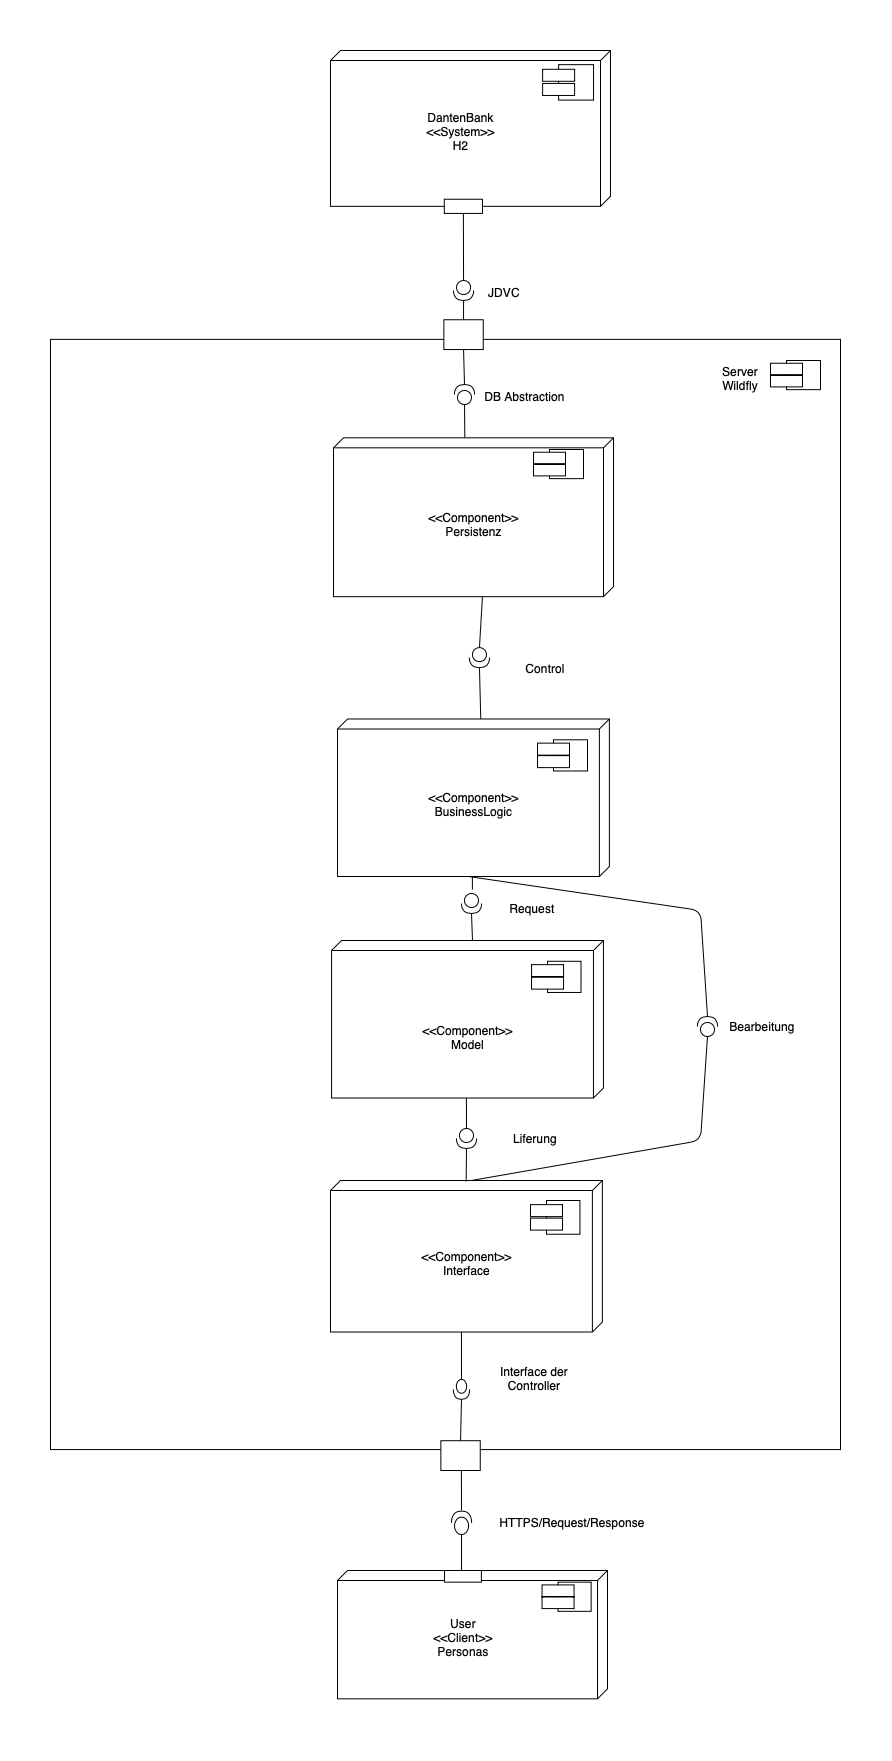
\includegraphics[width=310px]{UML/KonzeptioneleSicht.png}
  \caption{Die konzeptionelle Sicht}
  \label{fig:boat1}
\end{figure}

Figure \ref{fig:konzept} zeigt unsere konzeptionelle Sicht auf das System. 
Hierbei ist es wichtig zu bemerken, dass der Client abstract ist.
\section{Modulsicht}
\label{sec:modulsicht}

\subsection{Pakete}

\subsubsection{Model}

\subsubsection{Controller}

\subsubsection{Persistence}

\subsection{Module}


{\it
Diese Sicht beschreibt den statischen Aufbau des Systems mit Hilfe von
Modulen, Subsystemen, Schichten und Schnittstellen.
Diese Sicht ist hierarchisch, d.\,h. Module werden in Teilmodule
zerlegt. Die Zerlegung endet bei Modulen, die ein klar umrissenes
Arbeitspaket für eine Person darstellen und in einer Kalenderwoche
implementiert werden können. Die Modulbeschreibung der Blätter dieser
Hierarchie muss genau genug und ausreichend sein, um das Modul
implementieren zu können.

Die Modulsicht wird durch {UML}-Paket- und Klassendiagramme visualisiert.

Die Module werden durch ihre Schnittstellen beschrieben.
Die Schnittstelle eines Moduls $M$ ist die Menge aller Annahmen, die
andere Module über $M$ machen dürfen, bzw.\ jene Annahmen, die $M$
über seine verwendeten Module macht (bzw. seine Umgebung, wozu auch
Speicher, Laufzeit etc.\ gehören).
Konkrete Implementierungen dieser Schnittstellen sind das Geheimnis des Moduls
und können vom Programmierer festgelegt werden. Sie sollen hier
dementsprechend nicht beschrieben werden.

Die Diagramme der Modulsicht sollten die zur Schnittstelle gehörenden Methoden
enthalten. Die Beschreibung der einzelnen Methoden (im Sinne der Schnittstellenbeschreibung)
geschieht allerdings per Javadoc im zugehörigen Quelltext. Das bedeutet, dass Ihr
für alle Eure Module Klassen, Interfaces und Pakete erstellt und sie mit den Methoden der
Schnittstellen verseht. Natürlich noch ohne Methodenrümpfe bzw.\ mit minimalen Rümpfen.
Dieses Vorgehen vereinfacht den Schnittstellenentwurf und stellt Konsistenz sicher.

Jeder Schnittstelle liegt ein
Protokoll zugrunde. Das Protokoll beschreibt die Vor- und
Nachbedingungen der Schnittstellenelemente. Dazu gehören die erlaubten
Reihenfolgen, in denen Methoden der Schnittstelle aufgerufen werden
dürfen, sowie Annahmen über Eingabeparameter und Zusicherungen über
Ausgabeparameter. Das Protokoll von Modulen wird in der Modulsicht beschrieben.
Dort, wo es sinnvoll ist, sollte es mit Hilfe von Zustands- oder
Sequenzdiagrammen spezifiziert werden. Diese sind dann einzusetzen, wenn der
Text allein kein ausreichendes Verständnis vermittelt (insbesondere
bei komplexen oder nicht offensichtlichen Zusammenhängen).

Der Bezug zur konzeptionellen Sicht muss klar ersichtlich sein. Im
Zweifel sollte er explizit erklärt werden. Auch für diese Sicht muss
die Entstehung anhand der Strategien erläutert werden.
}




\section{Datensicht}
\label{sec:datensicht}

{ Zunächst existiert die Klasse Probe, welche die ID, die Legierung als (???), die Art der Behandlung und die Materialeigenschaften beinhaltet. Eine bestimmte Probe kann ausschließlich einem Träger zugeordnet werden. 
Die Klasse Träger besteht wieder aus einer ID, dem aktuellen Standort als  Standort und dem Typ als Trägerart. Ein Träger kann beliebig viele Proben beinhalten. Ein bestimmter Träger kann genau einer Experimentierstation (ES) zugeordnet sein. Eine Experimentierstation besteht aus einem Namen als String und dem Ort, an dem die ES zu finden ist als Standort. Einer bestimmten ES können beliebig viele Träger zugeordnet sein, während ihr immer nur ein  Technologe zugeordnet sein wird. Die ES ist immer nur einem bestimmten Prozessschritt (PS) zugeordnet. Ein Prozessschritt beinhaltet den Namen als String, die Prozessparameter (PP) als Prozessparameter, der Probenzustand, die Dauer und die Zustände und (???). Ein Prozessschritt ist einer bestimmten Prozesskette zugeordnet. Die Prozesskette (PK) beinhaltet den Namen als String. Sie beherbergt beliebig viele Prozessschritte und beliebig viele Prozesskettenaufträge. Der  Prozesskettenauftrag (PKAuftrag) kann nur einer Prozesskette zugeordnet sein und hat einen KettenInstanzwert (KIW) zugeordnet. \\}

{  Zunächst existiert die Klasse Probe, welche die ID, die Legierung als (???), die Art der Behandlung und die Materialeigenschaften beinhaltet. Eine bestimmte Probe kann ausschließlich einem Träger zugeordnet werden.
Die Klasse Träger besteht wieder aus einer ID, dem aktuellen Standort als  Standort und dem Typ als Trägerart. Ein Träger kann beliebig viele Proben beinhalten. Ein bestimmter Träger kann genau einer Experimentiertstation (ES) zugeordnet sein. Eine Experimentiertstation besteht aus einem Namen als String und dem Ort, an dem die ES zu finden ist als Standort. Einer bestimmten ES können beliebig viele Träger zugeordnet sein, während ihr immer nur einTechnologe zugeordnet sein wird. Die ES ist immer nur einem bestimmten Prozessschritt (PS) zugeordnet. Ein Prozessschritt beinhaltet den Namen als String, die Prozessparameter (PP) als Prozessparameter, der Probenzustand, die Dauer und die Zustände und (???). Ein Prozessschritt ist einer bestimmten Prozesskette zugeordnet. Die Prozesskette (PK) beinhaltet den Namen als String. Sie beherbergt beliebig viele Prozessschritte und beliebig viele Prozesskettenaufträge. Der  Prozesskettenauftrag (PKAuftrag) kann nur einer Prozesskette zugeordnet sein und hat einen KettenInstanzwert (KIW) zugeordnet. \\


Der Ketteninstanzwert ist einem PKAuftrag zugeordnet und beinhaltet beliebig viele Schnittinstanzwerte (SIW). Die Schnittinstanzwerte beinhalten einen Wert, welcher über KIW, PKAuftrag und die PK einem Prozessschritt zugeschrieben werden. Ein SIW kann einem KIW zugeordnet sein. 
Dies wird so gehandhabt, da man im Nachhinein, nachdem eine Prozesskette instanziiert wurde, die Werte noch einfach ändern können soll.
}

{\it Hier wird das der Anwendung zugrundeliegende Datenmodell
  beschrieben. Hierzu werden neben einem erläuternden Text auch ein
  oder mehrere {UML}-Klassendiagramme verwendet. Das hier beschriebene
  Datenmodell wird u.\,a. jenes der Anforderungsspezifikation enthalten,
  allerdings mit implementierungsspezifischen Änderungen und
  Erweiterungen. Siehe die gesonderten Hinweise.}
   
 \begin{sidewaysfigure}
  \caption{Datenmodell für DataColorado}
  \centering
  

  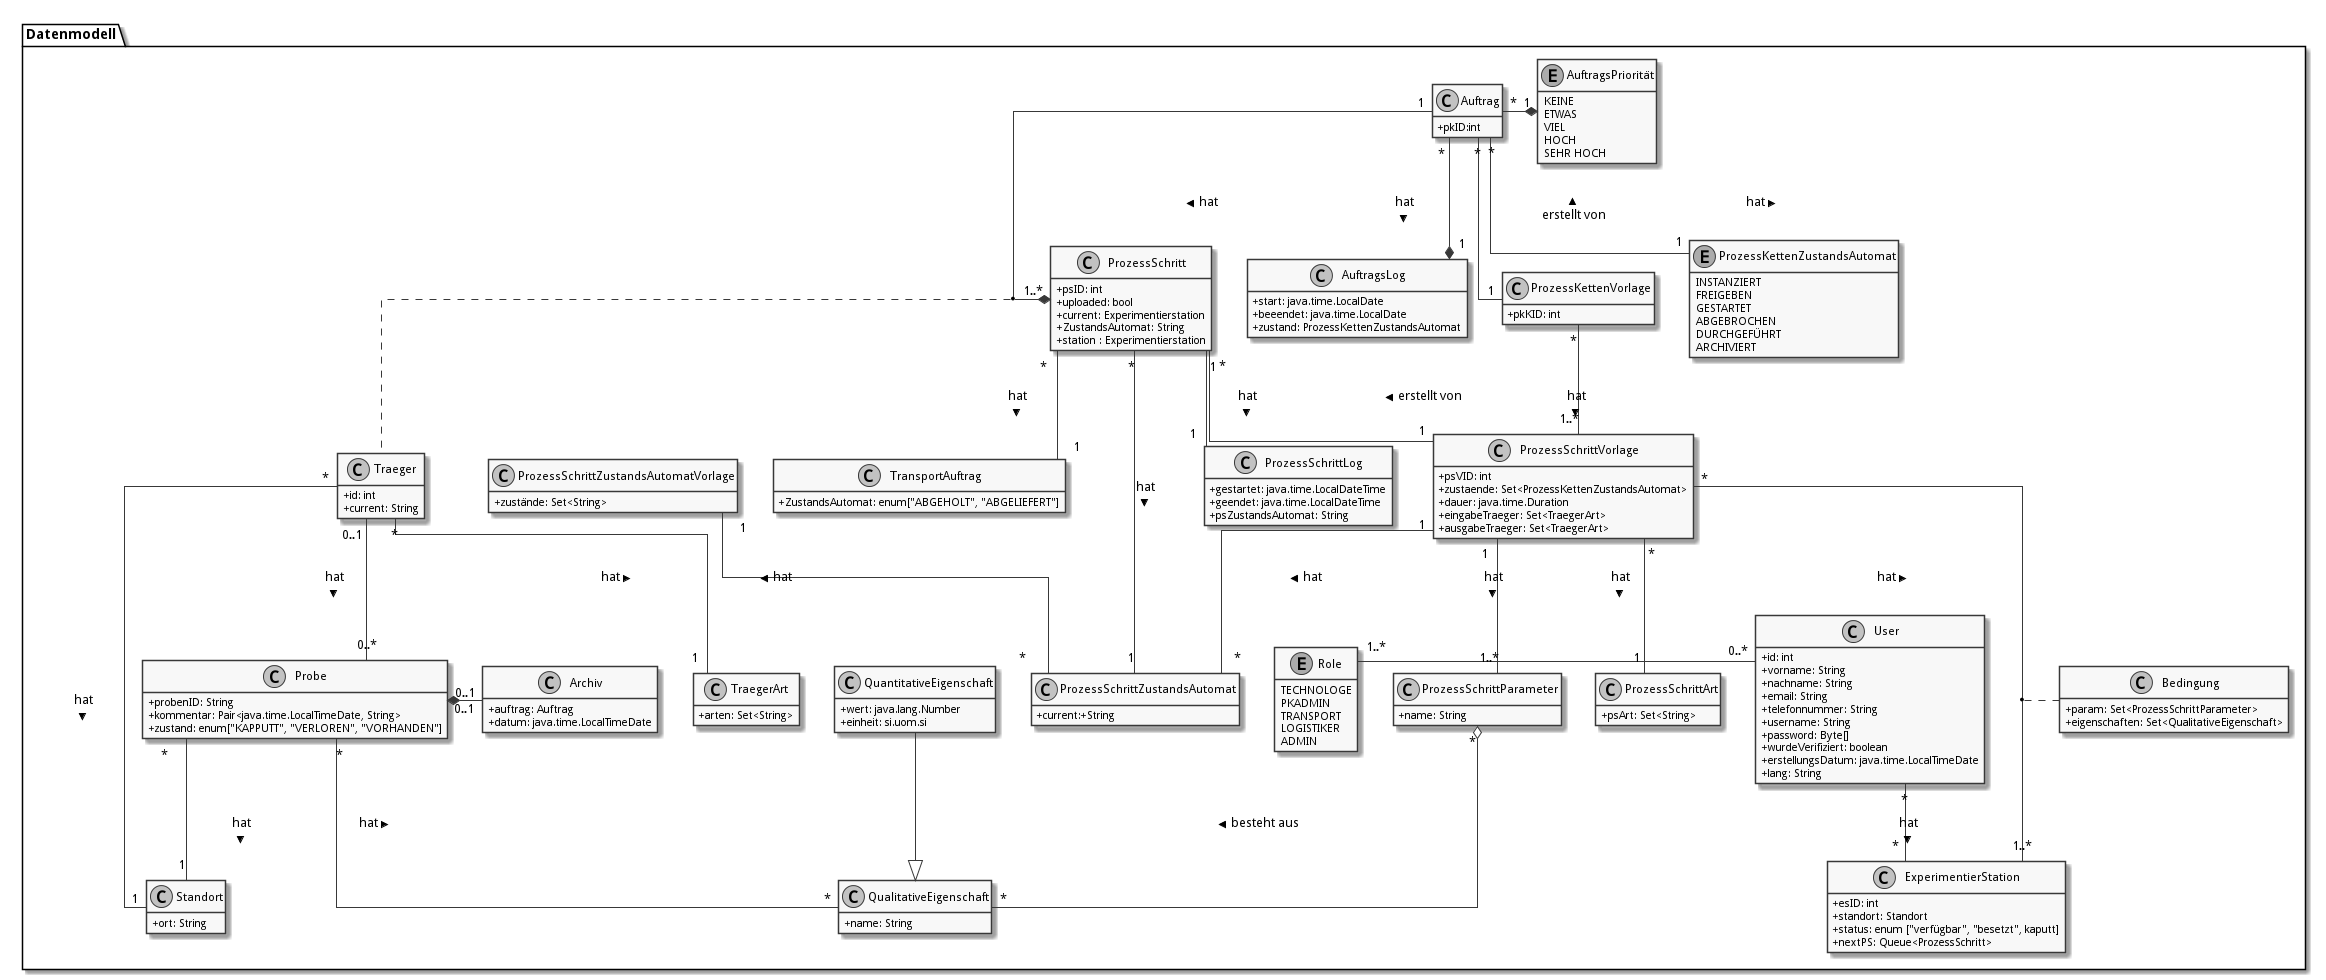
\includegraphics[width=0.75\textwidth]{UML/datenModel}

 \end{sidewaysfigure}

\section{Ausführungssicht}

\label{sec:ausfuehrung}


{ Im folgenden Schritt werden wir die Ausführungssicht erläutern. Es wird aufgezeigt, welche verschiedenen Geräte benötigt werden, welche Prozesse auf den Geräten jeweils laufen und welche Module dort enthalten sind.
}


%%\includepdf[]{06Ausfuehrungssicht.pdf}
\includegraphics[scale=0.5]{UML/06Ausfuehrungssicht.pdf}


{ Die Ausführungssicht von unserer Software (SWP2) ist in der obrigen Abbildung 6.1 modelliert.

Beliebig viele Benutzer können via TCP/IP auf den SFB-Server zugreifen. Dies geschieht über eine Webapplikation, die im Internetbrowser eines PCs oder eines mobilen Endgerät läuft.

Es gibt einen Anwendungsserver, welchen wir SFB-Server genannt haben, auf dem eine Instanz von Wildfly läuft. Auf dieser Wildflyinstanz wird der SWP2-Server mit allen dazugehörigen modulen ausgeführt.

Der SFB-Server stellt eine Verbindung über TCP/IP eine Verbindung zu dem einzigen Datenbankserver her. Auf dem Server läfut eine Instanz der Datenbanksoftware (........INSERT NAME...........).

}

{\it
Die Ausführungssicht beschreibt das Laufzeitverhalten. Hier
werden die Laufzeitelemente aufgeführt und beschrieben, welche Module
sie zur Ausführung bringen. Ein Modul kann von mehreren
Laufzeitelementen zur Laufzeit verwendet werden. Die Ausführungssicht
beschreibt darüber hinaus, welche Laufzeitelemente spezifisch
miteinander kommunizieren. Zudem wird bei verteilten Systemen
(z.\,B. Client-Server-Systeme) dargestellt, welche Module von welchen
Prozessen auf welchen Rechnern ausgeführt werden.}


\section[Zusammenhänge zwischen Anwendungsfällen und Architektur]{Zusammenhänge zwischen Anwendungsfällen und Architektur\sectionmark{Zusammenhänge AF u. Architektur}}
\sectionmark{Zusammenhänge AF u. Architektur}
\label{sec:anwendungsfaelle}


\subsection{Nutzer Verwalten}
\begin{figure}
  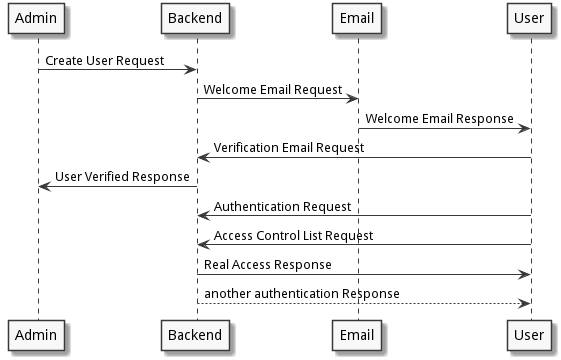
\includegraphics[width=\linewidth]{UML/seq.png}
  \caption{Anlegen eines Nutzers}
  \label{fig:pkErstellen}
\end{figure}
In dieser Graphik wird ein Nutzer vom Admin angelegt. Dieser muss dann eine Mail bestätigen und kann dann zugriff beantragen


\begin{figure}
  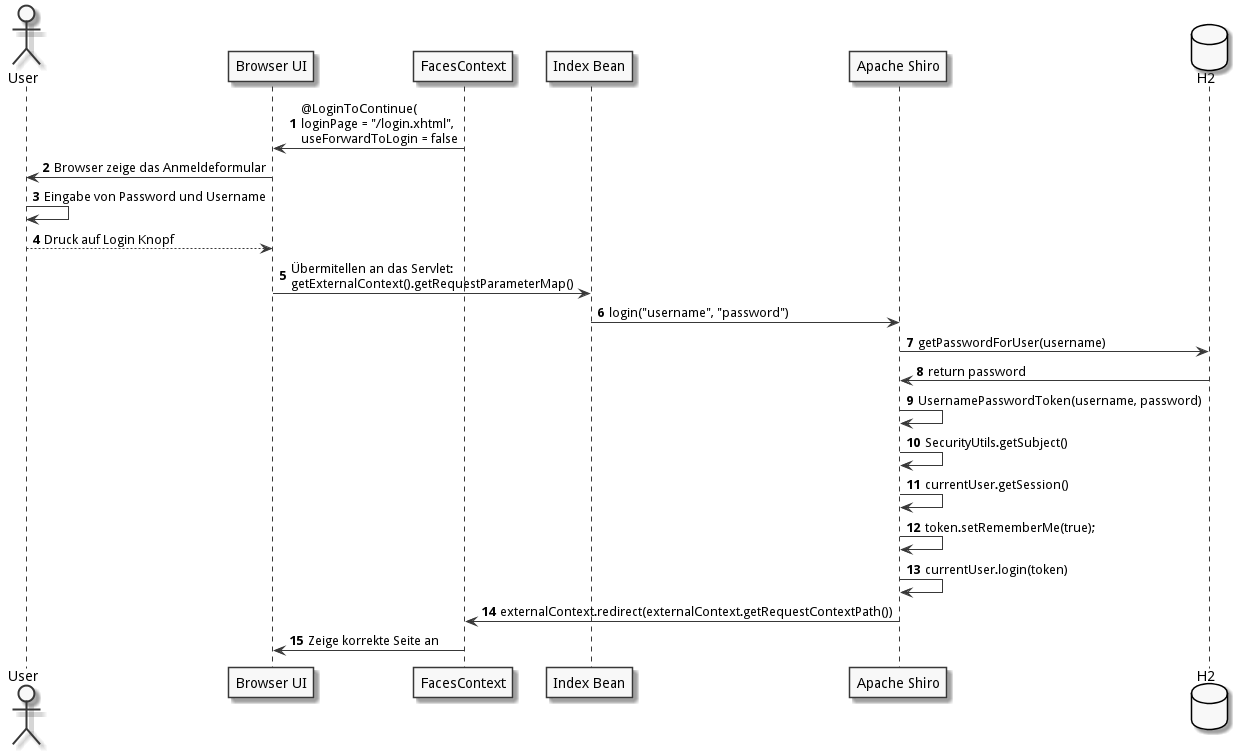
\includegraphics[width=\linewidth]{UML/erstbenutzung.png}
  \caption{Nutzer möchte sich auf dem System anmelden}
  \label{fig:pkErstellen}
\end{figure}
In dieser Graphik wird in einem Sequenzdiagramm gezeigt, wie der Nutzer sich auf unserem System anmelden kann. Dazu ruft er die Login Seite auf, meldet sich an und landet dann auf der richtigen Seite

\subsection{Prozessketten Verwalten und Proben beantragen}

\begin{figure}
  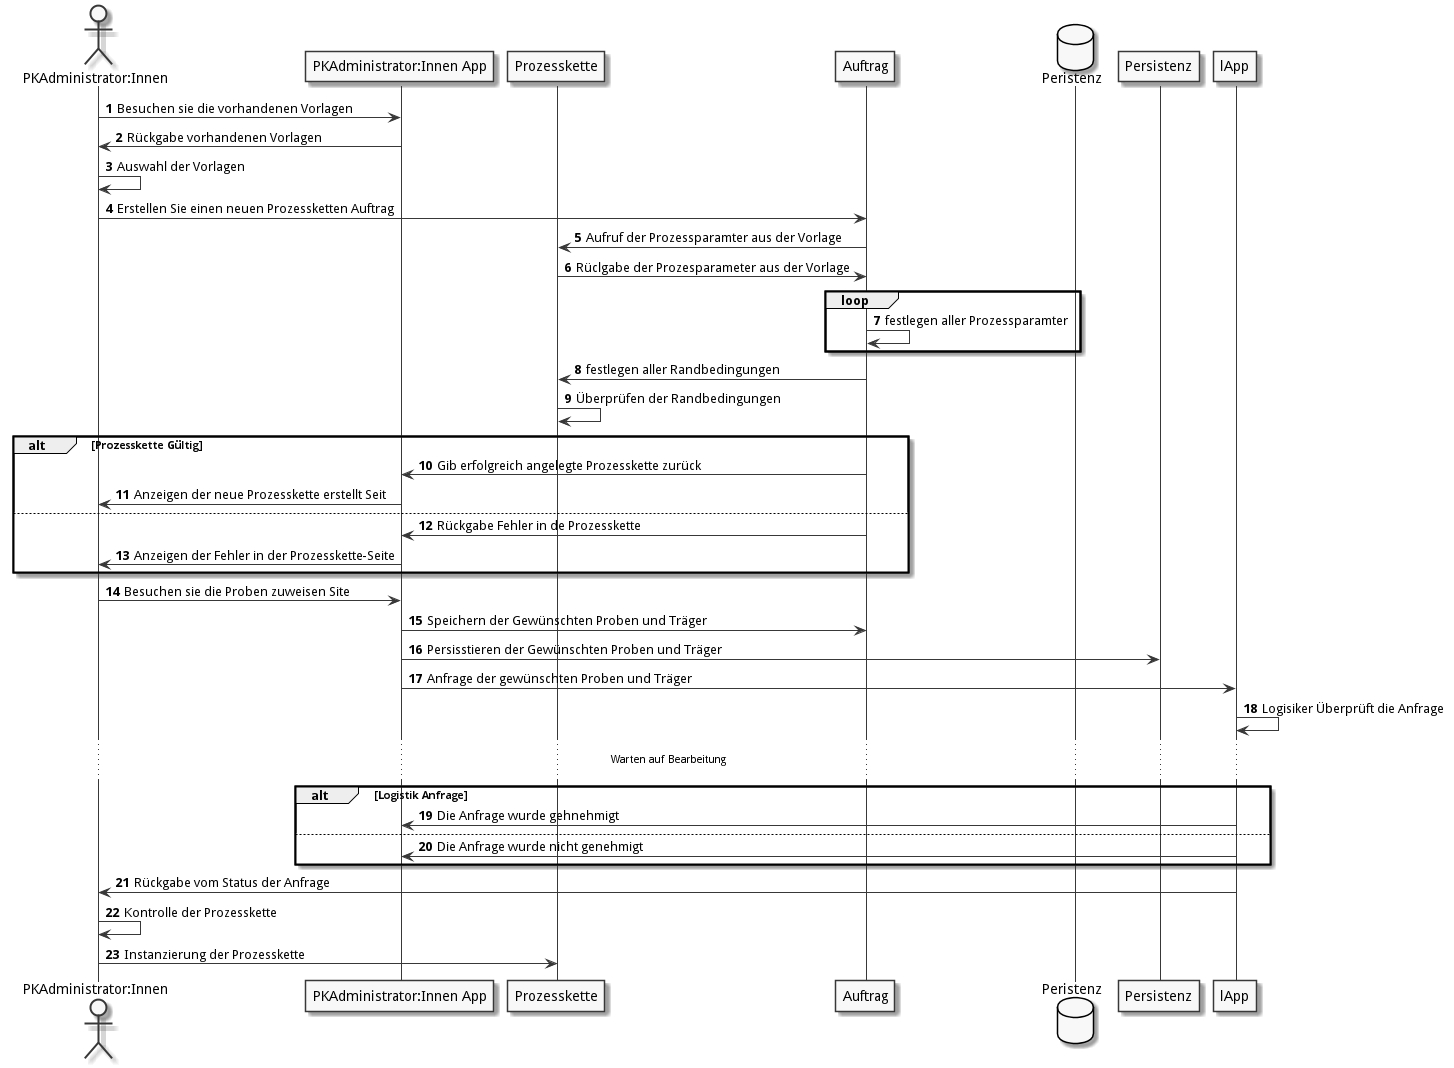
\includegraphics[width=\linewidth]{UML/pkErstellen.png}
  \caption{Ablauf des Erstellens einer Prozesskette}
  \label{fig:pkErstellen}
\end{figure}

Figure \ref{fig:pkErstellen} zeigt wie der Prozesskettenadministrator die Prozesskette erstellt. 
Bei Schritt 18, schauen sie bitte in Graphik \ref{fig:logstikProbenPüftZuweisen}. 

Der Prozesskettenadministrator wählt aus den vorhandenen Vorlagen eine aus, damit erstellt er einen neuen Auftrag und legt für diese alle Parameter fest.
Falls die Randbedingen der Kette stimmen darf diese instanziiert werden. Beim Speichern des Auftrages mit der instanzierten Prozesskette werden diese auch persistiert.

Jetzt erhält der Logistiker einen neuen Probenzuweisung Auftrag, falls die Anfrage genehmigt wurde kann der PKAdmin nun die Prozesskette starten

\begin{figure}
  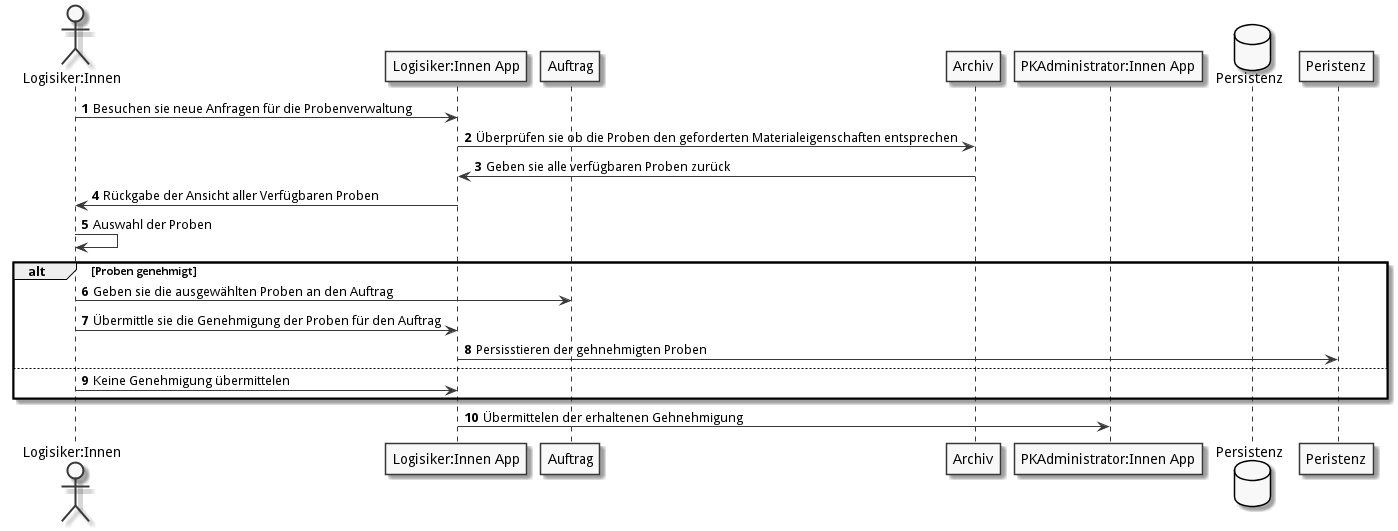
\includegraphics[width=\linewidth]{UML/logstikProbenPueftZuweisen.png}
  \caption{Ablauf vom zuweisen der Proben zu einer Prozessketteninstanz}
  \label{fig:logstikProbenPüftZuweisen}
\end{figure}

In der Graphik \ref{fig:logstikProbenPüftZuweisen} erhält die Logistik eine Anfrage für die Probenverwaltung. Es muss nun vom System geprüft werden ob Proben mit den gewünschten Materialeigenschaften im Lager sind. Das System gibt diese an die Logistik zurück. Werden die Proben dann von dem Logistiker ausgewählt und genehmigt, so werden diese an den Auftrag übermittelt und persistiert. Die Genehmigung wird an die Prozesskettenverwaltungs-Administrationsapp übermittelt.

\subsection{Proben Transport}
\subsection{Prozessschritt Ausführen}
\subsection{Lager Verwaltung}



{\it In diesem Abschnitt sollen Sequenzdiagramme mit Beschreibung(!)
  für zwei bis drei von Euch ausgewählte
    Anwendungsfälle
  erstellt werden. Ein Sequenzdiagramm beschreibt den
  Nachrichtenverkehr zwischen allen Modulen, die an der Realisierung
  des Anwendungsfalles beteiligt sind.  Wählt die
    Anwendungsfälle so, dass nach Möglichkeit alle Module Eures
    entworfenen Systems in mindestens einem Sequenzdiagramm
    vorkommen. Falls Euch das nicht gelingt, versucht möglichst viele
    und die wichtigsten Module abzudecken. }

\section{Evolution}

\label{sec:evolution}

\subsection{Kristallkugel Software}
{
Die erste Idee zum sinnvollen Erweitern der Software soll eine gewisse Vorraussicht ausgeben können, was nach einem beliebigen Schritt mit den Eigenschaften einer Probe passiert, bzw welche Eigenschaften die Proba danach wahrscheinlich haben wird. Das ganze soll durch einen analytischen Algorithmus realisiert werden, welcher die vorherigen Daten auswertet und daraus dann eine wahrscheinlichkeit für die Eigenschaften entwickelt und die wahrscheinlichsten Eigenschaften dann ausgibt. 
}
\subsection{Vorraussichtliche Dauer eines Prozesses}
{
Man kann den Algorithmus aus der Kristallkugel Software auch dafür verwenden, dass aus empirischen Daten die vorraussichtliche Dauer eines Prozesses errechnet und ausgegeben wird. 

Außerdem könnte man statt eines Algorithmus Microchips in die Experimentierstationen einbauen, welche die verbleibene Zeit an die Software weitergeben können. 
}
\subsection{Scanner}
{
Da so gut wie jedes mobile Endgerät eine Kamera besitzt, könnte man diese nutzen, um QR-Codes, die auf den Proben, den Trägern, im Archiv und an jeder Station zu finden sind, zu scannen damit z.B. der Transporter nichtmehr manuell eingeben muss, welche Datei er wohin bringt. \\
Er scannt den QR-Code des Trägers und dann die QR-Codes beliebig vieler Proben. Die Software ordnet nun automatisch die gescannten Proben dem gescannten Träger zu. 
Er kann den QR-Code des Trägers scannen und die Software weiß automatisch, dass der angemeldete Transporter den Träger abgeholt hat und wenn er jetzt den QR-Code der nächsten Experimentierstation scannt, trägt die Software automatisch den Träger als Abgeliefert ein. 
}

{\it
  Beschreibt in diesem Abschnitt, welche Änderungen Ihr
  vornehmen müsst, wenn sich Anforderungen oder Rahmenbedingungen
  ändern. Insbesondere würden hierbei die in der
  Anforderungsspezifikation unter "`Ausblick"' genannten
  Punkte behandelt werden.}

\dots


\end{document}


%%% Local Variables:
%%% mode: latex
%%% mode: reftex
%%% mode: flyspell
%%% ispell-local-dictionary: "de_DE"
%%% TeX-master: t
%%% End:
